\documentclass[11pt,a4paper,oneside]{report}

% ---------- codificación, idioma, tipografía ----------
\usepackage[utf8]{inputenc}
\usepackage[T1]{fontenc}
\usepackage{lmodern}
\usepackage[main=spanish,provide=*]{babel}
\emergencystretch=2em
\setlocalecaption{spanish}{table}{Tabla}
\setlocalecaption{spanish}{lot}{Índice de tablas}
\setlocalecaption{spanish}{lof}{Índice de figuras}
\setlocalecaption{spanish}{figure}{Figura}
\usepackage[a4paper,top=2.5cm,bottom=2.4cm,left=2.6cm,right=2.6cm]{geometry}
\usepackage{microtype}
\usepackage{setspace}
\setstretch{1.08}

% ---------- matemáticas ----------
\usepackage{amsmath,amssymb,mathtools}
\usepackage{bm}

% ---------- tablas, listas, figuras ----------
\usepackage{booktabs,array,tabularx,longtable}
\usepackage{enumitem}
\usepackage{graphicx}
\usepackage{xcolor}
\usepackage{caption}
\usepackage{float}
\usepackage{titlesec}
\usepackage{fancyhdr}
\usepackage{tikz}
\usepackage[most]{tcolorbox}
\usepackage[colorlinks=true,linkcolor=azulIPN,citecolor=azulIPN,urlcolor=azulIPN,bookmarksnumbered]{hyperref}

% ---------- colores (paleta azul y rojo) ----------
\definecolor{azulIPN}{HTML}{1F4E9C}
\definecolor{azulclaro}{HTML}{E8EEF9}
\definecolor{rojoIPN}{HTML}{C23B2E}
\definecolor{rojoclaro}{HTML}{FBEDEB}
\definecolor{grisIPN}{HTML}{5A6475}

% ---------- cajas ----------
\newtcolorbox{ideaclave}[1][Idea clave]{enhanced,breakable,colback=azulclaro,colframe=azulIPN,
  fonttitle=\bfseries\sffamily,title={#1},boxrule=0.6pt,arc=2pt,left=8pt,right=8pt,top=5pt,bottom=5pt,before skip=10pt,after skip=10pt}
\newtcolorbox{definicion}[1][Definición]{enhanced,breakable,colback=white,colframe=azulIPN,
  fonttitle=\bfseries\sffamily,title={#1},boxrule=0.6pt,arc=2pt,left=8pt,right=8pt,top=5pt,bottom=5pt,before skip=10pt,after skip=10pt}
\newtcolorbox{ejemplo}[1][Ejemplo con datos reales]{enhanced,breakable,colback=white,colframe=grisIPN,
  fonttitle=\bfseries\sffamily,title={#1},boxrule=0.6pt,arc=2pt,left=8pt,right=8pt,top=5pt,bottom=5pt,before skip=10pt,after skip=10pt}
\newtcolorbox{cuidado}[1][Cuidado]{enhanced,breakable,colback=rojoclaro,colframe=rojoIPN,
  fonttitle=\bfseries\sffamily,title={#1},boxrule=0.6pt,arc=2pt,left=8pt,right=8pt,top=5pt,bottom=5pt,before skip=10pt,after skip=10pt}

% ---------- títulos ----------
\titleformat{\chapter}[hang]{\sffamily\bfseries\LARGE\color{azulIPN}}{\thechapter}{0.7em}{}[{\color{azulIPN}\titlerule}]
\titlespacing*{\chapter}{0pt}{-6pt}{18pt}
\titleformat{\section}{\sffamily\bfseries\Large\color{azulIPN}}{\thesection}{0.6em}{}
\titleformat{\subsection}{\sffamily\bfseries\large\color{grisIPN}}{\thesubsection}{0.6em}{}
\captionsetup{font=small,labelfont={bf,sf},labelsep=period}
\setlist[itemize]{itemsep=2pt,topsep=4pt}
\setlist[enumerate]{itemsep=2pt,topsep=4pt}
\renewcommand{\arraystretch}{1.18}

% ---------- encabezado y pie ----------
\setlength{\headheight}{14pt}
\pagestyle{fancy}
\fancyhf{}
\fancyhead[L]{\small\sffamily\color{grisIPN}Calendario de quemas}
\fancyhead[R]{\small\sffamily\color{grisIPN}\leftmark}
\fancyfoot[C]{\small\sffamily\thepage}
\renewcommand{\headrulewidth}{0.3pt}
\renewcommand{\chaptermark}[1]{\markboth{\thechapter.\ #1}{}}
\fancypagestyle{plain}{\fancyhf{}\fancyfoot[C]{\small\sffamily\thepage}\renewcommand{\headrulewidth}{0pt}}

% ---------- macros ----------
\newcommand{\E}{\mathbb{E}}
\newcommand{\Var}{\operatorname{Var}}
\newcommand{\CV}{\operatorname{CV}}
\newcommand{\Pois}{\operatorname{Pois}}
\newcommand{\Bin}{\operatorname{Bin}}
\newcommand{\Beta}{\operatorname{Beta}}
\newcommand{\WAPE}{\ensuremath{\operatorname{WAPE}}}
\newcommand{\ind}{\mathbb{1}}
\newcommand{\dato}{\texttt{data}}
\DeclareMathOperator*{\argmax}{arg\,max}

% ---------- números generados desde los resultados ----------
\newcommand{\terraSM}{11.5}\newcommand{\terraNM}{4.6}\newcommand{\terraAN}{3.0}\newcommand{\terraSesgo}{-0.08}

\newcommand{\pisoSM}{5.0}\newcommand{\pisoAN}{0.4}

\newcommand{\totalArm}{1\,558\,720}\newcommand{\razonVM}{3.88}\newcommand{\difArm}{0.12}\newcommand{\crec}{11.9}


\begin{document}
\begin{titlepage}
\thispagestyle{empty}
\setlength{\parindent}{0pt}
\newgeometry{margin=2.4cm}
\begin{tikzpicture}[remember picture,overlay]
  \fill[azulIPN] (current page.north west) rectangle ([yshift=-5.2cm]current page.north east);
  \fill[rojoIPN] ([yshift=-5.2cm]current page.north west) rectangle ([yshift=-5.35cm]current page.north east);
  \node[anchor=north west,text=white,align=left,inner sep=0pt,font=\sffamily] at ([xshift=2.4cm,yshift=-1.5cm]current page.north west)
    {{\Large\bfseries Instituto Politécnico Nacional}\\[5pt]
     {\large Campus Puebla}\\[22pt]
     {\small NASA Space Apps Challenge 2026 \textbullet\ Reto «MODIS and VIIRS Hot Spots»}};
\end{tikzpicture}\par
\vspace*{3.9cm}

{\sffamily\bfseries\fontsize{30}{34}\selectfont\color{azulIPN} Calendario de quemas}\\[10pt]
{\sffamily\Large\color{grisIPN} Armonización de hotspots MODIS y VIIRS y pronóstico para México, 2000--2025}

\vspace{1.0cm}
{\sffamily\bfseries\large\color{rojoIPN} Procedimiento matemático y análisis estadístico}\\[4pt]
{\sffamily\color{grisIPN} Documento técnico para el equipo: cada fórmula se deduce paso a paso, se justifica y se interpreta.}

\vfill
\begin{tcolorbox}[colback=azulclaro,colframe=azulclaro,arc=3pt,left=12pt,right=12pt,top=10pt,bottom=10pt]
{\sffamily\bfseries\color{azulIPN} Equipo}\\[4pt]
\sffamily
Marcos Rodolfo Macías Mondragón\\
Lina Ariel Limón Cortés\\
Joel Morales Gutierrez\\
Alejandro David Zacatelco Escobar
\end{tcolorbox}

\vspace{0.6cm}
{\sffamily\color{grisIPN} Puebla, Puebla \;\textbullet\; noviembre de 2026}
\restoregeometry
\end{titlepage}


\pagenumbering{roman}
\setcounter{page}{1}
\tableofcontents
\clearpage
\listoffigures
\listoftables
\clearpage
\pagenumbering{arabic}
\setcounter{page}{1}

\chapter{Cómo leer este documento}

Este documento explica, con todo el detalle matemático y estadístico, qué hicimos en el proyecto «Calendario de quemas» y por qué cada decisión es razonable. Está escrito para que cualquier compañero del equipo pueda entender el procedimiento sin haber escrito el código, y para que pueda defenderlo ante preguntas del jurado.

\section{El proyecto en una página}

El reto pide una serie de hotspots (detecciones de fuego activo desde el espacio) que sea comparable entre los dos sensores de la NASA, MODIS y VIIRS, una aplicación web para explorarla y un calendario de quemas. Nuestro trabajo tiene tres partes que se apoyan una en la otra:

\begin{enumerate}[label=\arabic*)]
  \item \textbf{Armonización} (capítulos~\ref{cap:problema} a~\ref{cap:serie}). VIIRS cuenta casi cuatro veces más hotspots que MODIS porque ve con más resolución. Para tener una sola serie, convertimos cada detección de VIIRS en una fracción de «hotspot equivalente a MODIS», con un peso $k$ estimado por estado y por mes.
  \item \textbf{Validación} (capítulos~\ref{cap:valid} y~\ref{cap:result}). Medimos qué tan bien reproduce la serie armonizada a MODIS en años que el método no utilizó para calibrarse.
  \item \textbf{Pronóstico} (capítulo~\ref{cap:pron}). Un modelo deliberadamente sencillo (climatología más un ajuste de nivel que se apaga con el horizonte), con intervalos empíricos y una prueba hacia atrás honesta.
\end{enumerate}

\begin{ideaclave}[Los cuatro resultados que hay que recordar]
\begin{enumerate}[label=\arabic*.]
  \item La serie armonizada reproduce a MODIS con un error anual nacional de $1.3\,\%$ (un año fuera, 2012--2019) y de $2.1\,\%$ (años no vistos, 2020--2025).
  \item Calibrar por estado y por mes baja el error por estado y mes de $24.8\,\%$ a $12.9\,\%$ (un año fuera) y de $21.3\,\%$ a $14.5\,\%$ (años no vistos), frente a un factor único para todo México.
  \item Dos ideas que parecían buenas (fusionar píxeles de VIIRS y filtrar por potencia radiativa) empeoraron el resultado y se descartaron.
  \item A escala nacional el pronóstico empata con la climatología y supera con claridad a «igual que el año pasado»; no predice incendios y su valor para 2026 no se pudo verificar.
\end{enumerate}
\end{ideaclave}

\section{Convenciones}

\begin{itemize}
  \item Todas las cifras de este documento salen de los archivos del paquete (\texttt{validacion.json}, las series armonizadas y los resultados de la prueba hacia atrás). Las tablas se generaron con un script a partir de esos archivos, no se teclearon a mano. Los números que reproducimos de nuevo a partir de los CSV publicados coinciden con los del archivo de validación.
  \item Cuando decimos «error» sin más, nos referimos al error porcentual absoluto ponderado, \WAPE, definido en la sección~\ref{sec:wape}.
  \item Los cuadros de color tienen un significado fijo: azul para la idea que hay que quedarse; blanco con borde azul para definiciones; gris para ejemplos con datos reales; rojo para advertencias y límites.
  \item Los símbolos se resumen en la tabla~\ref{tab:simbolos}. Dos letras griegas se parecen y conviene no confundirlas: $\tau$ es el parámetro de contracción de la calibración (valor 100) y $\vartheta$ es la constante de decaimiento del pronóstico (valor 60 días). En el código ambas se llaman \texttt{tau}.
\end{itemize}

\begin{table}[H]
\centering
\caption{Símbolos principales.}\label{tab:simbolos}
\small
\begin{tabularx}{\textwidth}{@{}lX@{}}
\toprule
Símbolo & Significado \\
\midrule
$y,\;m,\;s$ & Año, mes del año ($1,\dots,12$) y estado ($s=1,\dots,32$). \\
$M_{y,m,s}$ & Número de hotspots de MODIS (Terra más Aqua) tras el filtro común. \\
$T_{y,m,s}$, $A_{y,m,s}$ & Lo mismo, solo Terra y solo Aqua. Se cumple $M=T+A$. \\
$V_{y,m,s}$ & Número de detecciones de VIIRS S-NPP tras el filtro común. \\
$k_{m,s}$ & Factor de calibración: hotspots de MODIS por cada detección de VIIRS en el estado $s$ y el mes $m$. \\
$k^{V}_{m,s},\;k^{T}_{m,s}$ & Factor de VIIRS a MODIS y factor de Terra a Terra más Aqua. \\
$\widehat{k},\;\widetilde{k}$ & Estimador por razón y estimador con contracción. \\
$\tau$ & Intensidad de la contracción en la calibración ($\tau=100$). \\
$w_i$ & Peso de la detección $i$ en la serie armonizada. \\
$H_{y,m,s}$ & Hotspots equivalentes a MODIS (serie armonizada). \\
$S_t$ & Serie diaria de una región en el día $t$ (base del pronóstico). \\
$T_0$ & Origen del pronóstico: último día observado. \\
$K,\;\lambda,\;W$ & Años de historia, peso de los años y semiancho de la ventana de la climatología. \\
$L,\;c_0$ & Días del ajuste de nivel y pseudoconteo de la razón de nivel. \\
$\vartheta$ & Constante de decaimiento del ajuste de nivel ($\vartheta=60$ días). \\
$\kappa$ & Pseudoconteo por día del error relativo del intervalo ($\kappa=0.5$). \\
\bottomrule
\end{tabularx}
\end{table}

\section{Ruta de lectura según lo que se necesite}

\begin{description}[leftmargin=1.2em,style=nextline]
  \item[Para exponer el proyecto en cinco minutos.] Capítulo~\ref{cap:problema}, secciones~\ref{sec:est-razon} y~\ref{sec:contraccion}, y los resultados del capítulo~\ref{cap:result}.
  \item[Para defender el método ante preguntas.] Capítulo~\ref{cap:valid} completo y el capítulo~\ref{cap:limites}, que dice con franqueza dónde puede fallar lo que hicimos.
  \item[Para reproducir o modificar el código.] Capítulo~\ref{cap:repro}.
\end{description}

\chapter{Datos y preparación}\label{cap:datos}

\section{Fuente y sensores}

Los datos son detecciones de fuego activo del sistema FIRMS de la NASA para México. Hay dos familias de sensores:

\begin{itemize}
  \item \textbf{MODIS}, a bordo de los satélites \emph{Terra} (desde noviembre de 2000) y \emph{Aqua} (desde julio de 2002). Cada píxel mide aproximadamente $1\times1$ km en el nadir.
  \item \textbf{VIIRS}, a bordo del satélite \emph{Suomi NPP} (S-NPP), desde enero de 2012. Su píxel es de 375 m, por eso detecta fuegos más pequeños.
\end{itemize}

Cada detección (\emph{hotspot}) es un píxel con una anomalía térmica. No es un incendio ni una superficie quemada: un mismo incendio grande produce muchos hotspots, y un fuego pequeño puede producir uno solo o ninguno. Esta advertencia vuelve en el capítulo~\ref{cap:limites}.

\section{Variables utilizadas}

De cada registro usamos la fecha de adquisición, la hora, la latitud y la longitud, el satélite, el tipo de fuente (\texttt{type}), la confianza (\texttt{confidence}), el indicador día o noche (\texttt{daynight}) y la potencia radiativa del fuego (\texttt{frp}, en megavatios). Para cargar los archivos y unificar los esquemas de los dos sensores usamos el \texttt{pipeline/01\_load.py}; el resto del procesamiento parte de ese archivo unificado, al que en el código nos referimos como \dato.

\section{Filtro común}

Para que los dos sensores cuenten lo mismo aplicamos exactamente el mismo filtro a todos los datos:

\begin{enumerate}[label=\arabic*)]
  \item \textbf{Tipo de fuente igual a 0}, es decir, presunto fuego de vegetación. Se descartan volcanes activos, fuentes estáticas y fuegos costa afuera.
  \item \textbf{Confianza nominal o alta}. En MODIS la confianza es un número de 0 a 100: usamos $\geq 30$ (nominal es de 30 a 79 y alta, de 80 en adelante). En VIIRS la confianza es una clase (\texttt{l}, \texttt{n}, \texttt{h}): usamos \texttt{n} y \texttt{h}.
  \item \textbf{Fecha hasta el 31 de diciembre de 2025}. Los datos de 2026 no entran.
\end{enumerate}

\begin{cuidado}[Por qué importa el filtro]
Si el filtro fuera distinto en cada sensor, parte de la diferencia entre MODIS y VIIRS vendría de reglas de selección y no del instrumento. El factor $k$ del capítulo~\ref{cap:factor} corrige la diferencia de instrumento \emph{dado} un filtro común; con otro filtro habría que volver a estimarlo.
\end{cuidado}

\section{Asignación a estados}

Cada detección se asigna a una entidad federativa con una cuadrícula auxiliar de $0.01^\circ$ (unos 1.1 km), con origen en $(-118^\circ,\,14^\circ)$. El procedimiento es:

\begin{enumerate}[label=\arabic*)]
  \item Se calcula la celda $(i_x,i_y)$ de cada detección con $i_x=\lfloor (\text{lon}+118)/0.01\rfloor$ e $i_y=\lfloor (\text{lat}-14)/0.01\rfloor$.
  \item Se asigna a cada celda distinta el estado cuyo polígono contiene su centro (contornos geoBoundaries gbOpen, nivel ADM1).
  \item Las celdas cuyo centro cae fuera de todo polígono (casi siempre por la línea de costa) se asignan al estado más cercano. El programa comprueba que la distancia máxima sea menor de 5 km.
\end{enumerate}

Asignar celdas y no puntos es una cuestión práctica: hay millones de detecciones pero solo unas decenas de miles de celdas distintas, y así los polígonos se consultan pocas veces.

\section{Conteos}

\begin{table}[H]
\centering
\caption{Detecciones que pasan el filtro común (noviembre de 2000 a diciembre de 2025).}\label{tab:conteos}
\begin{tabular}{@{}lr@{}}
\toprule
Sensor & Detecciones \\
\midrule
MODIS Terra & 702\,139 \\
MODIS Aqua & 790\,630 \\
VIIRS S-NPP & 3\,236\,119 \\
\midrule
Total filtrado & 4\,728\,888

\\
\bottomrule
\end{tabular}
\end{table}

Los 25 años y 2 meses de la serie son 9\,192 días. Con 32 estados, la tabla estado--día tiene $9\,192\times 32=294\,144$ renglones.

\section{De las detecciones a matrices de conteos}

Todo el análisis de la calibración trabaja con conteos mensuales por estado. Definimos, para cada año $y$, mes $m$ y estado $s$,
\begin{align*}
  T_{y,m,s}&=\#\{\text{detecciones de Terra}\},&
  A_{y,m,s}&=\#\{\text{detecciones de Aqua}\},\\
  V_{y,m,s}&=\#\{\text{detecciones de S-NPP}\},&
  M_{y,m,s}&=T_{y,m,s}+A_{y,m,s}.
\end{align*}
Son tres arreglos de dimensión $26\times12\times32$ (años 2000 a 2025). Con $M$ como referencia de «lo que MODIS habría contado», el objetivo del capítulo~\ref{cap:factor} es encontrar cómo convertir $V$ en algo comparable con $M$.

\begin{ideaclave}[Idea clave del capítulo]
Todo parte de una regla de selección común (vegetación, confianza nominal o alta) y de un conteo mensual por estado para cada sensor. Con esos tres arreglos, $M$, $V$ y $T$, se hace todo lo demás.
\end{ideaclave}

\chapter{El problema: dos sensores, dos formas de contar}\label{cap:problema}

\section{La diferencia es de instrumento, no de fuego}

Si sumamos todos los hotspots filtrados de 2013 a 2025, VIIRS cuenta \razonVM{} veces lo que cuenta MODIS en México. Una razón tan grande no puede venir de que haya más fuego en la zona que ve VIIRS, porque ambos sensores observan el mismo territorio. Viene de tres diferencias de instrumento:

\begin{enumerate}[label=\arabic*)]
  \item \textbf{Resolución espacial}: 375 m contra 1 km. Un fuego pequeño que no alcanza a calentar un píxel de 1 km puede encender uno de 375 m.
  \item \textbf{Hora de paso} del satélite sobre cada lugar, que cambia el estado del fuego observado y la cantidad de nubes y de humo.
  \item \textbf{Algoritmo de detección}, con umbrales distintos.
\end{enumerate}

Si pegáramos las dos series tal cual, la serie «saltaría» cuatro veces hacia arriba en 2012 y parecería que las quemas se cuadruplicaron. No es cierto: cambió el instrumento.

\begin{figure}[H]
\centering
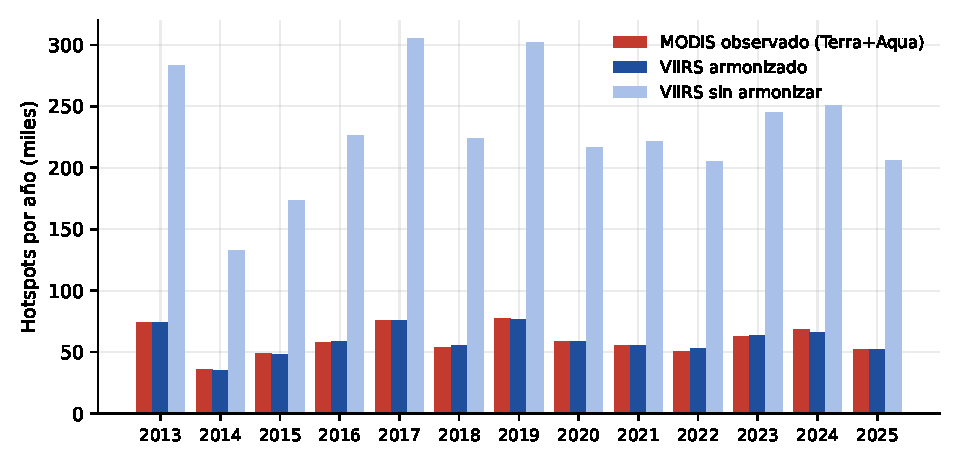
\includegraphics[width=0.95\textwidth]{fig/fig_anual.pdf}
\caption{Hotspots anuales en México, 2013--2025. La barra clara (VIIRS sin armonizar) queda casi cuatro veces por encima de MODIS. Después de armonizar, la barra azul prácticamente coincide con la roja. El factor se calibró con 2012--2019, de modo que el ajuste de 2020 en adelante es fuera de muestra.}\label{fig:anual}
\end{figure}

\section{Qué significa «armonizar»}

La figura~\ref{fig:anual} ya anticipa el objetivo. Queremos asignar a cada detección $i$ de VIIRS un peso $w_i\geq0$ tal que, en cualquier región y mes, la suma de pesos reproduzca \emph{en promedio} lo que habría contado MODIS. Con la notación del capítulo~\ref{cap:datos}, si $H_{y,m,s}=\sum_{i\in(y,m,s)} w_i$ es la suma de pesos,
\begin{align*}
  \E\!\left[H_{y,m,s}\right] &= \E\!\left[M_{y,m,s}\right].
\end{align*}
Esta es la propiedad que queremos y, además, la que verificamos con datos que el método no vio (capítulo~\ref{cap:valid}).

\begin{definicion}[Unidad común: el hotspot equivalente a MODIS]
Un \emph{hotspot equivalente a MODIS} es lo que habrían contado Terra y Aqua juntos. Una detección de VIIRS vale $k<1$ hotspots equivalentes, porque VIIRS cuenta más que MODIS. Una detección de MODIS posterior a julio de 2002 vale 1 hasta que empieza VIIRS (sección~\ref{sec:etapas}).
\end{definicion}

\section{Por qué el factor depende del estado y del mes}

Si la razón entre lo que cuentan los dos sensores fuera la misma siempre y en todas partes, bastaría un número único. No lo es, porque la razón depende de cuántos fuegos pequeños hay (que cambia con el tipo de vegetación y con la temporada) y de las nubes y del humo (que cambian con la estación). La figura~\ref{fig:knat} muestra que, incluso a escala nacional, la razón de MODIS entre VIIRS pasa de $0.19$ en junio a $0.31$ en diciembre. El capítulo~\ref{cap:result} cuantifica cuánto mejora el resultado al permitir esa variación.

\begin{figure}[H]
\centering
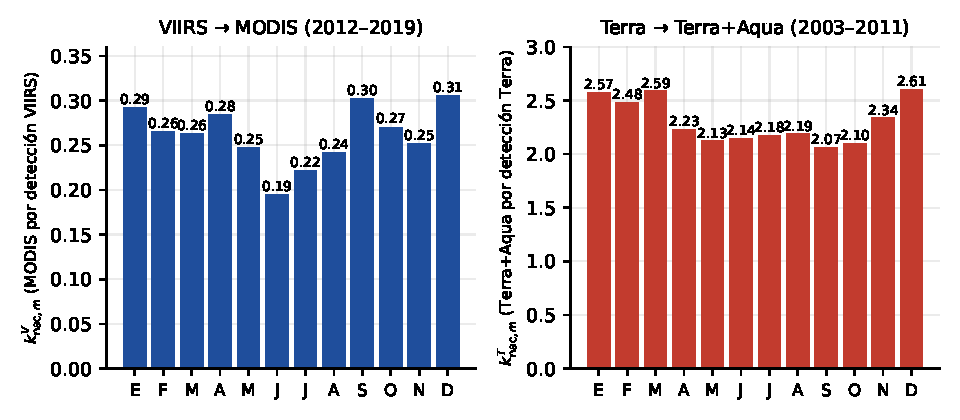
\includegraphics[width=0.98\textwidth]{fig/fig_knat.pdf}
\caption{Factor nacional por mes. Izquierda: hotspots de MODIS por cada detección de VIIRS (calibración 2012--2019). Derecha: hotspots de Terra más Aqua por cada detección de Terra (calibración 2003--2011).}\label{fig:knat}
\end{figure}

\begin{ideaclave}[Idea clave del capítulo]
VIIRS cuenta \razonVM{} veces más que MODIS por razones de instrumento. Armonizar consiste en dar a cada detección de VIIRS un peso $k$ menor que 1, de modo que la suma de pesos reproduzca lo que habría contado MODIS. El peso varía con el estado y con el mes del año.
\end{ideaclave}

\chapter{El factor de calibración}\label{cap:factor}

Este es el corazón matemático del proyecto. Primero deducimos por qué el estimador natural del factor es una razón de totales (sección~\ref{sec:est-razon}); después medimos su incertidumbre (sección~\ref{sec:var}); luego lo mejoramos con una contracción hacia el valor nacional (sección~\ref{sec:contraccion}), y finalmente justificamos el valor del parámetro de la contracción (sección~\ref{sec:tau}).

\section{Un modelo sencillo para los conteos}\label{sec:modelo}

Fijemos un estado $s$ y un mes del año $m$. Para cada año $y$ de entrenamiento tenemos dos conteos, $M_y$ (MODIS) y $V_y$ (VIIRS). Los conteos son números enteros no negativos que cuentan eventos poco frecuentes por celda de espacio-tiempo, así que el modelo de referencia es de Poisson. Suponemos
\begin{align*}
  V_y\sim\Pois(\mu_y),\qquad M_y\sim\Pois(k\,\mu_y),\qquad V_y\perp M_y\mid \mu_y,
\end{align*}
donde $\mu_y>0$ es la intensidad de detección de VIIRS en ese año y $k>0$ es el factor que buscamos: \emph{MODIS cuenta en promedio $k$ veces lo que cuenta VIIRS}, $\E[M_y]=k\,\E[V_y]$.

Hay dos observaciones importantes sobre el modelo:

\begin{itemize}
  \item La intensidad $\mu_y$ cambia libremente de un año a otro (hay años de mucho fuego y años de poco). Es un \emph{parámetro de estorbo}: no nos interesa, pero no podemos suponerlo constante.
  \item El factor $k$ es el mismo todos los años dentro de la celda estado--mes. Esa es la hipótesis sustantiva: la relación entre los instrumentos es estable, aunque el fuego no lo sea.
\end{itemize}

\section{El estimador por razón}\label{sec:est-razon}

\subsection{Deducción por máxima verosimilitud condicional}

Queremos estimar $k$ sin tener que estimar los $\mu_y$. La clave es condicionar al total $N_y=M_y+V_y$. Si dos variables de Poisson independientes tienen medias $a$ y $b$, condicional a su suma $N$ la primera sigue una binomial:
\begin{align*}
  \Pr(M=j\mid N=n)
  &=\frac{\Pr(M=j)\Pr(V=n-j)}{\Pr(N=n)}
  =\frac{e^{-k\mu}\frac{(k\mu)^j}{j!}\;e^{-\mu}\frac{\mu^{n-j}}{(n-j)!}}{e^{-(1+k)\mu}\frac{((1+k)\mu)^n}{n!}}\\[4pt]
  &=\binom{n}{j}\left(\frac{k}{1+k}\right)^{j}\left(\frac{1}{1+k}\right)^{n-j}.
\end{align*}
El resultado no depende de $\mu$: la intensidad desaparece. Por lo tanto, condicional a los totales $N_y$,
\begin{align*}
  M_y\mid N_y\sim\Bin\!\left(N_y,\;p\right),\qquad p=\frac{k}{1+k}.
\end{align*}
Esta es una probabilidad que tiene una lectura directa: $p$ es la proporción de las detecciones totales (MODIS más VIIRS) que corresponden a MODIS.

Con los $n$ años de entrenamiento, la log-verosimilitud condicional es, salvo constantes,
\begin{align*}
  \ell(p)=\Big(\sum_y M_y\Big)\log p+\Big(\sum_y V_y\Big)\log(1-p).
\end{align*}
Derivamos e igualamos a cero:
\begin{align*}
  \frac{d\ell}{dp}=\frac{\sum_y M_y}{p}-\frac{\sum_y V_y}{1-p}=0
  \quad\Longrightarrow\quad
  \widehat{p}=\frac{\sum_y M_y}{\sum_y M_y+\sum_y V_y}.
\end{align*}
Como $k=p/(1-p)$ y la máxima verosimilitud es invariante a reparametrizaciones,
\begin{align}
  \boxed{\;\widehat{k}=\frac{\widehat p}{1-\widehat p}=\frac{\sum_y M_y}{\sum_y V_y}\;}\label{eq:khat}
\end{align}

\begin{ideaclave}
El factor de calibración es el cociente de los totales de entrenamiento: hotspots de MODIS entre detecciones de VIIRS. Se obtiene sin necesidad de modelar cuánto fuego hubo cada año.
\end{ideaclave}

\subsection{Por qué razón de totales y no promedio de razones}

Otra opción sería calcular la razón de cada año, $M_y/V_y$, y promediarlas. No lo hacemos por dos motivos. Primero, el cociente~\eqref{eq:khat} es un promedio ponderado de las razones anuales con pesos proporcionales a $V_y$:
\begin{align*}
  \widehat{k}=\frac{\sum_y M_y}{\sum_y V_y}=\sum_y\frac{V_y}{\sum_j V_j}\cdot\frac{M_y}{V_y},
\end{align*}
de modo que los años con más información cuentan más. Segundo, el promedio simple de razones se descontrola cuando algún $V_y$ es pequeño: una razón $M_y/V_y$ calculada con $V_y=2$ es muy ruidosa y pesaría igual que una calculada con $V_y=20\,000$.

\section{Qué tan incierto es el factor}\label{sec:var}

Sea $N=\sum_y N_y$ el total de detecciones de entrenamiento. Condicional a los $N_y$, la suma $\sum_y M_y$ es suma de binomiales independientes con la misma $p$, así que es binomial de parámetros $(N,p)$. Entonces $\Var(\widehat p)=p(1-p)/N$. Como $k=g(p)=p/(1-p)$ y $g'(p)=1/(1-p)^2$, el método delta da
\begin{align*}
  \Var(\widehat k)\approx g'(p)^2\Var(\widehat p)
  =\frac{p(1-p)}{N(1-p)^4}=\frac{p}{N(1-p)^3}.
\end{align*}
Sustituimos $p=k/(1+k)$, de modo que $1-p=1/(1+k)$, y $\E[N]=(1+k)\sum_y\mu_y=(1+k)\sum_y\E[V_y]$:
\begin{align*}
  \Var(\widehat k)\approx\frac{k(1+k)^{2}}{(1+k)\sum_y \mu_y}=\frac{k(1+k)}{\sum_y\mu_y}.
\end{align*}
El error relativo, el coeficiente de variación, queda muy sencillo:
\begin{align}
  \CV(\widehat k)^2=\frac{\Var(\widehat k)}{k^2}\approx\frac{1+k}{k\sum_y\mu_y}
  =\frac{1}{\sum_y \mu_y}+\frac{1}{k\sum_y\mu_y}
  \approx\frac{1}{\sum_y V_y}+\frac{1}{\sum_y M_y}.\label{eq:cv}
\end{align}
Es la varianza relativa de una razón de dos conteos de Poisson: cada conteo aporta el inverso de su tamaño.

\begin{ejemplo}[Cuánta incertidumbre hay en dos celdas reales]
Guerrero en mayo (2012--2019) tiene $\sum M=26\,402$ y $\sum V=113\,412$. Entonces $\CV\approx\sqrt{1/26\,402+1/113\,412}\approx0.7\,\%$: el factor está bien determinado. Tlaxcala en noviembre tiene $\sum M=6$ y $\sum V=22$, así que $\CV\approx\sqrt{1/6+1/22}\approx46\,\%$: el factor es casi un volado. El mismo procedimiento da una precisión de $0.7\,\%$ en una celda y de $46\,\%$ en otra.
\end{ejemplo}

\begin{cuidado}[La fórmula es un piso de la incertidumbre]
La ecuación~\eqref{eq:cv} supone conteos de Poisson independientes. Los fuegos reales se agrupan en el espacio y en el tiempo (un incendio grande genera cientos de hotspots), por lo que los conteos están \emph{sobredispersos} y la incertidumbre real es mayor. Por eso la usamos como una cota inferior y como justificación cualitativa de la contracción, no como un intervalo de confianza.
\end{cuidado}

\section{Contracción hacia el factor nacional}\label{sec:contraccion}

El ejemplo anterior muestra el problema: en celdas con pocos datos, $\widehat k_{m,s}$ es muy ruidoso. La figura~\ref{fig:contraccion} lo corrige con una idea que ya aparece en otras partes de la estadística: pedir prestada fuerza al conjunto. En lugar de $\widehat k_{m,s}$ usamos
\begin{align}
  \boxed{\;\widetilde k_{m,s}=\frac{\sum_{y}M_{y,m,s}+\tau\,\widehat k_{\mathrm{nac},m}}{\sum_{y}V_{y,m,s}+\tau}\;},\qquad
  \widehat k_{\mathrm{nac},m}=\frac{\sum_{y}\sum_{s}M_{y,m,s}}{\sum_{y}\sum_{s}V_{y,m,s}},\label{eq:ktilde}
\end{align}
con $\tau=100$. El factor nacional del mes, $\widehat k_{\mathrm{nac},m}$, es el mismo estimador de la ecuación~\eqref{eq:khat} aplicado a todo el país.

\subsection{Tres lecturas equivalentes}

\paragraph{1) Pseudoconteos.} Es como agregar $\tau$ detecciones de VIIRS «ficticias» a la celda, acompañadas de $\tau\,\widehat k_{\mathrm{nac},m}$ hotspots de MODIS ficticios en la proporción nacional. Una celda con muchos datos apenas nota el agregado; una celda con pocos datos queda dominada por él.

\paragraph{2) Promedio ponderado.} Se factoriza el numerador:
\begin{align*}
  \widetilde k_{m,s}
  =\frac{\sum_y V_{y,m,s}}{\sum_y V_{y,m,s}+\tau}\cdot\underbrace{\frac{\sum_y M_{y,m,s}}{\sum_y V_{y,m,s}}}_{\widehat k_{m,s}}
  +\frac{\tau}{\sum_y V_{y,m,s}+\tau}\cdot\widehat k_{\mathrm{nac},m}
  =\omega\,\widehat k_{m,s}+(1-\omega)\,\widehat k_{\mathrm{nac},m},
\end{align*}
con peso propio $\omega=\sum_yV_{y,m,s}/(\sum_yV_{y,m,s}+\tau)\in(0,1)$. Con $\sum V=\tau$ el estado cuenta la mitad; con $\sum V\gg\tau$ prevalece su propio dato; con $\sum V\ll\tau$ prevalece el nacional.

\paragraph{3) Estimador bayesiano.} Con la parametrización $p=k/(1+k)$ del capítulo anterior, tomemos una distribución a priori $p\sim\Beta(\alpha,\beta)$ con $\alpha=\tau\,\widehat k_{\mathrm{nac},m}$ y $\beta=\tau$, cuya media $\alpha/(\alpha+\beta)=\widehat k_{\mathrm{nac},m}/(1+\widehat k_{\mathrm{nac},m})$ es la proporción nacional. La media a posteriori de $p$ con $\sum M$ éxitos en $N$ ensayos es
\begin{align*}
  \widetilde p=\frac{\sum M+\alpha}{N+\alpha+\beta}=\frac{\sum M+\tau\,\widehat k_{\mathrm{nac},m}}{\sum M+\sum V+\tau(1+\widehat k_{\mathrm{nac},m})}.
\end{align*}
Al invertir la relación, $\widetilde p/(1-\widetilde p)$, el numerador se queda en $\sum M+\tau\widehat k_{\mathrm{nac},m}$ y el denominador en $\sum V+\tau$. Es exactamente la ecuación~\eqref{eq:ktilde}. Así que la contracción es la media a posteriori de la proporción de MODIS bajo una a priori centrada en el país, cuya fuerza equivale a $\tau$ observaciones.

\begin{figure}[H]
\centering
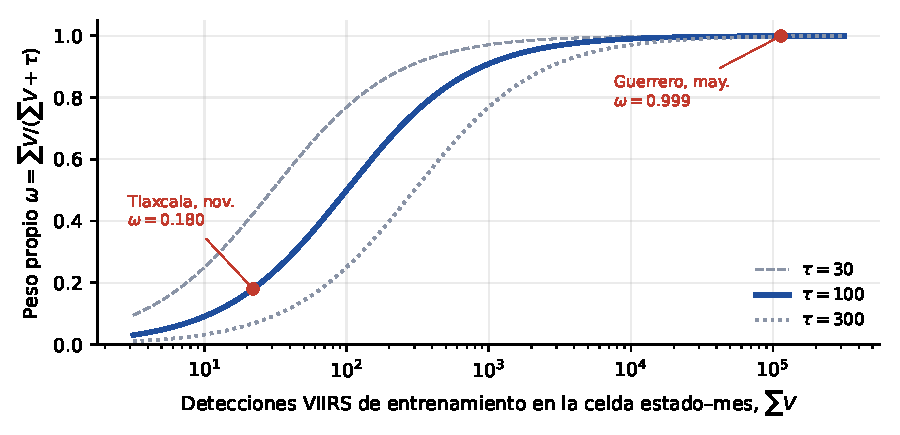
\includegraphics[width=0.85\textwidth]{fig/fig_contraccion.pdf}
\caption{Peso propio $\omega$ de una celda estado--mes según sus detecciones de VIIRS de entrenamiento. Con $\tau=100$, una celda con 22 detecciones (Tlaxcala en noviembre) pone solo $18\,\%$ en su propio dato; una celda con más de cien mil (Guerrero en mayo) pone prácticamente todo.}\label{fig:contraccion}
\end{figure}

\subsection{Ejemplos con datos reales}

\begin{table}[H]
\centering
\caption{Efecto de la contracción en cuatro celdas estado--mes (entrenamiento 2012--2019). $\widehat k$ es la razón de la ecuación~\eqref{eq:khat}; $\widetilde k$, la de la ecuación~\eqref{eq:ktilde}; CV es el piso de la ecuación~\eqref{eq:cv}.}\label{tab:ejemplos}
\small
\begin{tabular}{@{}lrrrrrrr@{}}
\toprule
Celda & $\sum M$ & $\sum V$ & $\widehat k$ & $\widehat k_{\mathrm{nac}}$ & $\omega$ & $\widetilde k$ & CV (\%) \\
\midrule
Tlaxcala (noviembre) & 6 & 22 & 0.273 & 0.251 & 0.180 & 0.255 & 46.1 \\
Aguascalientes (agosto) & 35 & 20 & 1.750 & 0.242 & 0.167 & 0.493 & 28.0 \\
Morelos (octubre) & 5 & 40 & 0.125 & 0.270 & 0.286 & 0.229 & 47.4 \\
Guerrero (mayo) & 26\,402 & 113\,412 & 0.233 & 0.247 & 0.999 & 0.233 & 0.7

\\
\bottomrule
\end{tabular}
\end{table}

En Aguascalientes en agosto, con 20 detecciones de VIIRS y 35 de MODIS, la razón propia ($1.75$) es siete veces el valor nacional ($0.24$): confiar en ella convertiría cada detección de VIIRS en casi dos hotspots equivalentes. La contracción la lleva a $0.49$. En cambio, en Guerrero en mayo el factor casi no se mueve. Esa es la conducta buscada: corregir donde hay ruido y respetar donde hay información.

\section{Elección de \texorpdfstring{$\tau$}{tau}}\label{sec:tau}

El parámetro $\tau$ se probó en la rejilla $\{0,10,30,100,300,1000\}$ con los dos ejercicios de validación del capítulo~\ref{cap:valid}. La tabla~\ref{tab:tau} la reproduce a partir de los CSV publicados.

\begin{table}[H]
\centering
\caption{Error de la calibración por estado y mes según $\tau$. Con $\tau=0$ no hay contracción. Valores en \%.}\label{tab:tau}
\small
\begin{tabular}{@{}rcccc@{}}
\toprule
 & \multicolumn{2}{c}{Error por estado y mes} & \multicolumn{2}{c}{Error anual nacional}\\
\cmidrule(lr){2-3}\cmidrule(lr){4-5}
$\tau$ & Un año fuera & Fuera de muestra & Un año fuera & Fuera de muestra \\
\midrule
0 & 13.0 & 14.9 & 1.2 & 2.6 \\
10 & 12.9 & 14.7 & 1.3 & 2.3 \\
30 & 12.9 & 14.6 & 1.3 & 2.2 \\
\textbf{100} & \textbf{12.9} & \textbf{14.5} & \textbf{1.3} & \textbf{2.1} \\
300 & 12.9 & 14.5 & 1.3 & 2.1 \\
1000 & 13.1 & 14.5 & 1.4 & 2.1

\\
\bottomrule
\end{tabular}
\end{table}

La conclusión es que la superficie de error es plana: entre $\tau=30$ y $\tau=300$ el error por estado y mes cambia en menos de dos décimas de punto porcentual en ambos ejercicios. Quitar toda la contracción ($\tau=0$) cuesta unos $0.4$ puntos porcentuales en el error fuera de muestra, y contraer demasiado ($\tau=1000$) empeora algo el ejercicio de un año fuera.

\begin{cuidado}[Una precisión de honestidad]
Elegimos $\tau=100$ comparando los dos ejercicios, incluido el de 2020--2025. Por eso ese conjunto no es del todo «virgen» para esta decisión. Como el efecto de $\tau$ es de décimas de punto y plano en un rango amplio, el sesgo de selección es pequeño, pero conviene decirlo. Los demás parámetros del capítulo~\ref{cap:pron} se ajustaron con otro criterio: solo con años anteriores a 2020.
\end{cuidado}

\section{Un detalle: enero de 2012}

VIIRS S-NPP empieza el 20 de enero de 2012. Por eso el mes de enero de 2012 está incompleto para VIIRS y se excluye al calibrar y al evaluar: se elimina de $\sum M$ y de $\sum V$ (y de los errores de la validación). Sin esta exclusión, enero tendría un factor artificialmente alto, porque MODIS cuenta el mes completo y VIIRS solo once días.

\begin{ideaclave}[Idea clave del capítulo]
El factor de calibración es una razón de totales, $\widehat k=\sum M/\sum V$, que sale de máxima verosimilitud condicional y no exige modelar la intensidad del fuego de cada año. Su error relativo es del orden de $\sqrt{1/\sum M+1/\sum V}$. Donde hay pocos datos, la contracción con $\tau=100$ lo acerca al valor nacional del mismo mes, y esa corrección equivale a una media a posteriori beta--binomial.
\end{ideaclave}

\chapter{Construcción de la serie armonizada}\label{cap:serie}

\section{Tres etapas, tres reglas de peso}\label{sec:etapas}

La cobertura de los sensores cambia con el tiempo, así que la serie se arma por etapas. Sea $d_i$ la fecha de la detección $i$.

\begin{definicion}[Pesos de la serie armonizada]
\begin{align*}
  w_i=\begin{cases}
    k^{T}_{m,s} & \text{si } i\text{ es de Terra y } d_i<\text{4 jul 2002 (etapa 1: solo Terra, escalada)},\\[2pt]
    1 & \text{si } i\text{ es de Terra o Aqua y } \text{4 jul 2002}\le d_i<\text{20 ene 2012 (etapa 2)},\\[2pt]
    k^{V}_{m,s} & \text{si } i\text{ es de S-NPP (etapa 3, desde el 20 de enero de 2012)},\\[2pt]
    0 & \text{si } i\text{ es de Terra o Aqua y } d_i\ge\text{20 ene 2012}.
  \end{cases}
\end{align*}
donde $m$ y $s$ son el mes y el estado de la detección $i$.
\end{definicion}

La serie en la unidad común es la suma de pesos,
\begin{align*}
  H_{y,m,s}=\sum_{i\in(y,m,s)}w_i.
\end{align*}

\begin{enumerate}[label=\arabic*)]
  \item \textbf{Etapa 1 (1 de noviembre de 2000 a 3 de julio de 2002).} Solo observa Terra. Para llevarla a la unidad de «Terra más Aqua» la multiplicamos por un factor $k^T_{m,s}$ calibrado con 2003--2011 (sección~\ref{sec:terra}).
  \item \textbf{Etapa 2 (4 de julio de 2002 a 19 de enero de 2012).} Ya observan Terra y Aqua, que es exactamente la unidad de referencia. Cada detección vale 1.
  \item \textbf{Etapa 3 (desde el 20 de enero de 2012).} Se usa VIIRS con el factor $k^{V}_{m,s}$ de la ecuación~\eqref{eq:ktilde}. MODIS deja de entrar a la serie y se conserva únicamente como referencia para validar.
\end{enumerate}

\begin{figure}[H]
\centering
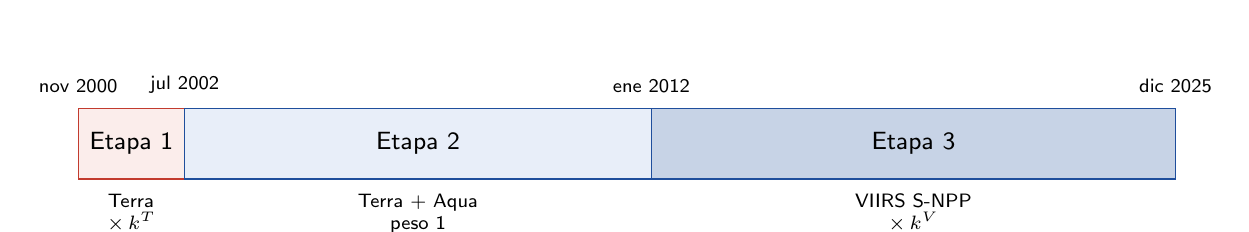
\begin{tikzpicture}[x=0.52cm,y=1cm,font=\small\sffamily]
  \def\a{0}\def\b{2.6}\def\c{14}\def\d{26.8}
  \fill[rojoclaro,draw=rojoIPN] (\a,0) rectangle (\b,0.9);
  \fill[azulclaro,draw=azulIPN] (\b,0) rectangle (\c,0.9);
  \fill[azulIPN!25,draw=azulIPN] (\c,0) rectangle (\d,0.9);
  \node at (1.3,0.45) {Etapa 1};\node at (8.3,0.45) {Etapa 2};\node at (20.4,0.45) {Etapa 3};
  \node[below=2pt,text width=2.4cm,align=center,font=\scriptsize\sffamily] at (1.3,0) {Terra\\ $\times\,k^{T}$};
  \node[below=2pt,align=center,font=\scriptsize\sffamily] at (8.3,0) {Terra + Aqua\\ peso 1};
  \node[below=2pt,align=center,font=\scriptsize\sffamily] at (20.4,0) {VIIRS S-NPP\\ $\times\,k^{V}$};
  \node[above=2pt,font=\scriptsize\sffamily] at (\a,0.9) {nov 2000};
  \node[above=2pt,font=\scriptsize\sffamily] at (\b,0.9) {jul 2002};
  \node[above=2pt,font=\scriptsize\sffamily] at (\c,0.9) {ene 2012};
  \node[above=2pt,font=\scriptsize\sffamily] at (\d,0.9) {dic 2025};
\end{tikzpicture}
\caption{Las tres etapas de la serie armonizada. La etapa 1 es la más incierta porque su factor se estima en años posteriores.}\label{fig:etapas}
\end{figure}

\section{Factor de Terra a Terra más Aqua}\label{sec:terra}

En la etapa 1 aplicamos la misma idea del capítulo~\ref{cap:factor} con otro par de conteos. Se calibra con los años en que Terra y Aqua operan completos y en que aún no hay VIIRS, 2003--2011:
\begin{align*}
  \widetilde k^{T}_{m,s}=\frac{\sum_{y=2003}^{2011}M_{y,m,s}+\tau\,\widehat k^{T}_{\mathrm{nac},m}}{\sum_{y=2003}^{2011}T_{y,m,s}+\tau},\qquad
  \widehat k^{T}_{\mathrm{nac},m}=\frac{\sum_y\sum_sM_{y,m,s}}{\sum_y\sum_sT_{y,m,s}}.
\end{align*}
Aquí $M=T+A$, de modo que el factor nacional es mayor que 2: Aqua cuenta un poco más que Terra, y el factor oscila entre $2.07$ y $2.61$ según el mes (figura~\ref{fig:knat}, derecha). Por tanto, a nivel nacional una detección de Terra en 2001 vale entre dos y tres hotspots equivalentes, según el mes.

\begin{cuidado}[La etapa 1 es una extrapolación hacia atrás]
El factor de Terra se calibra con 2003--2011 y se aplica a 2000--2002. Suponemos que la relación entre Terra y Terra más Aqua no cambió en esos años, algo que no podemos comprobar porque en esa etapa no hay un segundo sensor con el cual compararse. Por eso la presentamos como la parte más incierta de la serie. Su validación (sección~\ref{sec:val-terra}) solo comprueba que el método funciona \emph{dentro} del periodo en que sí se puede medir.
\end{cuidado}

\section{Resultado: la serie}

La serie armonizada tiene \totalArm{} hotspots equivalentes a MODIS entre noviembre de 2000 y diciembre de 2025. El año con más hotspots equivalentes es 2011 ($100\,017$) y el de menos, entre los años completos, es 2014 ($35\,372$). La tabla estado--mes y la tabla estado--día son las que descarga la aplicación.

\begin{ideaclave}[Idea clave del capítulo]
La serie usa tres reglas: Terra escalada hasta julio de 2002, Terra más Aqua con peso 1 hasta enero de 2012, y VIIRS con su factor desde entonces. En cualquiera de las tres, un hotspot equivalente es «lo que habría contado MODIS».
\end{ideaclave}

\chapter{Diseño de la validación}\label{cap:valid}

Una armonización que solo se mide en los datos con los que se calibró presume un acierto que no tiene: los parámetros ya «vieron» las respuestas. Este capítulo describe cómo medimos el error de forma honesta, y el capítulo~\ref{cap:result} muestra los resultados.

\section{La predicción que se evalúa}

Con los factores calibrados con un conjunto de años $\mathcal{E}$ (entrenamiento), la serie armonizada de un año $y\notin\mathcal{E}$ en la unidad común es
\begin{align*}
  \widehat H_{y,m,s}=\widetilde k_{m,s}^{(\mathcal{E})}\;V_{y,m,s},
\end{align*}
donde $\widetilde k^{(\mathcal{E})}_{m,s}$ se calculó con la ecuación~\eqref{eq:ktilde} usando solo los años de $\mathcal{E}$. La referencia es lo que MODIS observó, $M_{y,m,s}$. Medimos qué tan lejos queda $\widehat H$ de $M$.

\section{La métrica: error porcentual absoluto ponderado}\label{sec:wape}

\begin{definicion}[WAPE]
Para un conjunto de celdas $\mathcal{C}$ (por ejemplo, todas las combinaciones año--mes--estado de un periodo),
\begin{align*}
  \WAPE(\mathcal{C})=\frac{\sum_{i\in\mathcal{C}}\bigl|\widehat H_i-M_i\bigr|}{\sum_{i\in\mathcal{C}}M_i}.
\end{align*}
\end{definicion}

\paragraph{Por qué esta métrica.} Si $\mathrm{APE}_i=|\widehat H_i-M_i|/M_i$ es el error porcentual de cada celda, el WAPE es su promedio ponderado con pesos proporcionales al tamaño observado:
\begin{align*}
  \WAPE(\mathcal{C})=\sum_{i\in\mathcal{C}}\frac{M_i}{\sum_{j\in\mathcal{C}}M_j}\,\mathrm{APE}_i.
\end{align*}
Las celdas grandes pesan más y las celdas con $M_i=0$ no producen divisiones entre cero, algo que sí ocurre con el error porcentual absoluto medio (MAPE) en celdas con pocos fuegos. Además, tiene una interpretación inmediata: «de cada 100 hotspots de MODIS, nos equivocamos en $x$».

Se calcula en tres niveles de agregación, que responden a preguntas distintas:

\begin{enumerate}[label=\arabic*)]
  \item \textbf{Por estado y mes} (el más exigente): las celdas son $(y,m,s)$.
  \item \textbf{Nacional por mes}: primero se suma sobre los estados y luego se compara, $\bigl|\sum_s\widehat H_{y,m,s}-\sum_sM_{y,m,s}\bigr|$.
  \item \textbf{Nacional por año}: se suma sobre meses y estados,
    \begin{align*}
      \WAPE_{\text{anual}}=\frac{\sum_y\bigl|\sum_{m,s}(\widehat H_{y,m,s}-M_{y,m,s})\bigr|}{\sum_{y,m,s}M_{y,m,s}}.
    \end{align*}
\end{enumerate}

Además se reporta el \textbf{sesgo} relativo, $\sum(\widehat H-M)/\sum M$, que dice si la serie sistemáticamente sobreestima ($>0$) o subestima ($<0$), y la correlación entre las series mensuales nacionales.

\section{Dos ejercicios de validación}

\subsection{Un año fuera}

Se recorren los años de 2012 a 2019. Para cada año $y_0$ se calibra con los otros siete y se predice el año omitido; es la validación cruzada «dejar un año fuera» (\emph{leave-one-year-out}, LOYO). El error que se reporta es el promedio de las ocho evaluaciones:
\begin{align*}
  \overline{\WAPE}_{\mathrm{LOYO}}=\frac{1}{8}\sum_{y_0=2012}^{2019}\WAPE\Bigl(\{(y_0,m,s)\};\;\widetilde k^{(\{2012,\dots,2019\}\setminus\{y_0\})}\Bigr).
\end{align*}
Responde: ¿qué tan bien predice el método un año cuyo comportamiento no usó? Su debilidad es que los años omitidos son contemporáneos de los de entrenamiento.

\subsection{Años no vistos}

Se calibra con 2012--2019 y se evalúa en 2020--2025, seis años completos que el método jamás utilizó. Responde: ¿el factor sigue funcionando hacia el futuro? Es el ejercicio más cercano al uso real y, por ello, el que más peso tiene en las conclusiones. Su debilidad es que, al ser un solo bloque, es un único experimento.

\begin{ideaclave}[Por qué los dos]
El ejercicio de un año fuera usa mucha información (ocho evaluaciones) pero en años parecidos a los de calibración. El ejercicio de años no vistos usa una sola evaluación, pero hacia el futuro. Si el método anduviera bien en uno y mal en el otro, desconfiaríamos de él. Reportamos ambos y vemos que cuentan la misma historia.
\end{ideaclave}

\section{Cómo interpretar el nivel del error}\label{sec:piso}

Los errores por estado y mes ($\sim\!14\,\%$) son mucho mayores que los anuales nacionales ($\sim\!2\,\%$). Parte de esa diferencia es solo ruido de conteo. Para verlo, suponga que $\widehat k$ es el valor correcto del factor. Entonces el error de una celda, $e=kV-M$, con $V\sim\Pois(\mu)$ y $M\sim\Pois(k\mu)$ independientes, cumple
\begin{align*}
  \E[e]=0,\qquad \Var(e)=k^2\mu+k\mu=k(1+k)\,\mu.
\end{align*}
Si $e$ es aproximadamente normal, $\E|e|=\sqrt{2/\pi}\,\sqrt{\Var(e)}$. Sustituyendo $\mu$ por $V$ observada y sumando sobre las celdas, el \emph{piso de ruido} del WAPE por estado y mes es
\begin{align*}
  \WAPE_{\text{piso}}\approx\frac{\sqrt{2/\pi}\;\sum_{i}\sqrt{k_i(1+k_i)\,V_i}}{\sum_iM_i}.
\end{align*}
Para el nivel anual nacional el piso se calcula con la suma de las varianzas de todas las celdas del año, $\sqrt{2/\pi}\sum_y\sqrt{\sum_{m,s}k(1+k)V}/\sum M$, porque los errores de signo opuesto se compensan al sumar.

\begin{ejemplo}[Piso de ruido en 2020--2025]
Con los datos de los años no vistos, el piso es de \pisoSM{}\,\% por estado y mes y de \pisoAN{}\,\% anual nacional. Se observó $14.5\,\%$ y $2.1\,\%$. Así que alrededor de un tercio del error por estado y mes es ruido de Poisson inevitable; el resto (y casi todo el error anual) es variación sistemática del factor de un año a otro y sobredispersión.
\end{ejemplo}

Esta cuenta es una referencia de orden de magnitud, no una descomposición exacta: supone Poisson e independencia, y ya vimos que los conteos reales están sobredispersos.

\section{Qué comparamos}

\begin{enumerate}[label=\arabic*)]
  \item \textbf{Nivel de factor}: un factor único para todo México y todo el año; un factor por mes (nacional); o un factor por estado y mes con contracción.
  \item \textbf{Variantes del conteo de VIIRS}: fusionar los píxeles de VIIRS que caen dentro de la huella de 1 km, y descartar detecciones con baja potencia radiativa (FRP).
  \item \textbf{Terra a Terra más Aqua}, con la misma lógica de dejar un año fuera dentro de 2003--2011.
\end{enumerate}

Las variantes de conteo se construyen así. «Fusionar» conserva una sola detección por satélite, fecha, indicador día o noche y celda de $0.01^\circ$ (la de mayor FRP), para imitar el píxel de 1 km de MODIS; en la práctica solo afecta de manera apreciable a VIIRS. El umbral de FRP elimina las detecciones de VIIRS con potencia menor que 2, 4 o 6 MW. Ambas son ideas razonables (compensar la resolución de VIIRS) que ponemos a prueba, no suposiciones.

\begin{ideaclave}[Idea clave del capítulo]
Medimos el error con el WAPE en tres niveles (estado--mes, nacional--mes, nacional--año) y con dos ejercicios: dejar un año fuera (2012--2019) y predecir años que el método nunca vio (2020--2025). Una parte del error es ruido de Poisson que ningún método elimina; por eso las comparaciones entre métodos se hacen en los mismos datos.
\end{ideaclave}

\chapter{Resultados de la armonización}\label{cap:result}

\section{El nivel del factor importa}

La tabla~\ref{tab:niveles} compara los tres niveles del factor en los dos ejercicios. El factor por estado y mes con contracción reduce el error por estado y mes de $24.8\,\%$ a $12.9\,\%$ en el ejercicio de un año fuera, y de $21.3\,\%$ a $14.5\,\%$ en años no vistos: entre un tercio y la mitad menos error que con un factor único. El error anual nacional cae de $4.9\,\%$ a $1.3\,\%$ y de $3.3\,\%$ a $2.1\,\%$.

\begin{table}[H]
\centering
\caption{Error (WAPE, \%) por nivel del factor. «UF» es el ejercicio de un año fuera (2012--2019) y «NV», el de años no vistos (2020--2025).}\label{tab:niveles}
\small
\begin{tabular}{@{}lrrrrrr@{}}
\toprule
 & \multicolumn{2}{c}{Estado y mes} & \multicolumn{2}{c}{Nacional y mes} & \multicolumn{2}{c}{Nacional y año}\\
\cmidrule(lr){2-3}\cmidrule(lr){4-5}\cmidrule(lr){6-7}
Factor & UF & NV & UF & NV & UF & NV \\
\midrule
Factor único (todo México, todo el año) & 24.8 & 21.3 & 10.4 & 8.2 & 4.9 & 3.3 \\
Factor por mes (nacional) & 22.9 & 21.2 & 6.3 & 6.9 & 4.6 & 4.0 \\
Factor por estado y mes (contracción $\tau$=100) & 12.9 & 14.5 & 3.7 & 5.4 & 1.3 & 2.1

\\
\bottomrule
\end{tabular}
\end{table}

\begin{figure}[H]
\centering
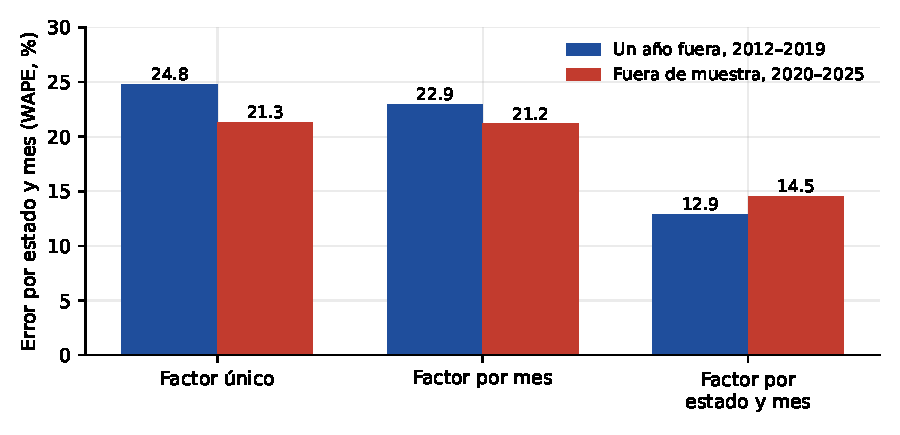
\includegraphics[width=0.85\textwidth]{fig/fig_niveles.pdf}
\caption{Error por estado y mes según el nivel del factor.}\label{fig:niveles}
\end{figure}

Hay dos lecturas distintas. El factor por mes (nacional) reduce mucho el error nacional por mes (de $10.4\,\%$ a $6.3\,\%$ en un año fuera) porque corrige la estacionalidad de la razón, pero apenas mejora el error por estado, porque no distingue entre estados. El factor por estado y mes corrige ambas cosas.

\begin{table}[H]
\centering
\caption{Sesgo relativo (\%) y correlación mensual nacional. UF: un año fuera; NV: años no vistos.}\label{tab:sesgo}
\small
\begin{tabular}{@{}lrrrr@{}}
\toprule
 & \multicolumn{2}{c}{Sesgo (\%)} & \multicolumn{2}{c}{Correlación mensual} \\
\cmidrule(lr){2-3}\cmidrule(lr){4-5}
Factor & UF & NV & UF & NV \\
\midrule
Factor único (todo México, todo el año) & $-$0.34 & $-$1.13 & 0.9921 & 0.9939 \\
Factor por mes (nacional) & $-$0.24 & $-$0.91 & 0.9990 & 0.9939 \\
Factor por estado y mes (contracción $\tau$=100) & $-$0.06 & 0.39 & 0.9993 & 0.9959

\\
\bottomrule
\end{tabular}
\end{table}

El sesgo de la serie armonizada es prácticamente cero: $-0.06\,\%$ en un año fuera y $+0.39\,\%$ en años no vistos para el factor elegido. Con los factores de 2012--2019, la suma 2013--2025 de VIIRS armonizado difiere de la de MODIS observado en solo \difArm{}\,\%. Ese número, ojo, \emph{no} es fuera de muestra: 2013--2019 pertenece al entrenamiento. Los ejercicios del capítulo anterior son los que valen para juzgar el método.

\section{Ideas sofisticadas que no ayudaron}

La tabla~\ref{tab:variantes} muestra las variantes de conteo de VIIRS. Fusionar los píxeles dentro de una huella de 1 km y filtrar por FRP son decisiones razonables, pero empeoran todas las métricas: el error anual fuera de muestra pasa de $2.1\,\%$ a entre $4.4\,\%$ y $7.6\,\%$ y aparece un sesgo negativo de hasta $-6.6\,\%$.

\begin{table}[H]
\centering
\caption{Variantes del conteo de VIIRS con factor por estado y mes. WAPE (\%) por estado y mes y anual nacional; sesgo en años no vistos. UF: un año fuera; NV: años no vistos.}\label{tab:variantes}
\small
\begin{tabular}{@{}lrrrrr@{}}
\toprule
 & \multicolumn{2}{c}{Estado y mes} & \multicolumn{2}{c}{Nacional y año} & Sesgo \\
\cmidrule(lr){2-3}\cmidrule(lr){4-5}\cmidrule(lr){6-6}
Variante & UF & NV & UF & NV & NV \\
\midrule
\textbf{Sin huella ni umbral de FRP (elegida)} & 12.9 & 14.5 & 1.3 & 2.1 & 0.4 \\
Con huella de 1 km (fusiona píxeles VIIRS) & 13.8 & 15.9 & 2.7 & 4.4 & $-$3.3 \\
Huella de 1 km $+$ FRP VIIRS $\geq$ 2 MW & 14.8 & 16.1 & 4.8 & 6.9 & $-$5.9 \\
Huella de 1 km $+$ FRP VIIRS $\geq$ 4 MW & 15.1 & 16.3 & 4.8 & 7.6 & $-$6.6 \\
Huella de 1 km $+$ FRP VIIRS $\geq$ 6 MW & 14.7 & 15.6 & 3.8 & 6.8 & $-$5.4

\\
\bottomrule
\end{tabular}
\end{table}

¿Por qué empeoran? Una explicación plausible, que no probamos por separado, es que la razón entre sensores se estima \emph{para el conteo que se usa}. Al recortar o fusionar, el conteo de VIIRS pierde fuegos que MODIS sí ve en proporciones que cambian entre años; el factor ya no es estable y la calibración no lo absorbe. El resultado que sí está medido es el comparativo: no ayudan, así que la solución simple gana.

\section{Terra a Terra más Aqua}\label{sec:val-terra}

Con la misma lógica de dejar un año fuera, dentro de 2003--2011, el factor de Terra a Terra más Aqua tiene un error de \terraSM{}\,\% por estado y mes, \terraNM{}\,\% nacional por mes y \terraAN{}\,\% anual, con sesgo $\terraSesgo\,\%$. Frente al factor de VIIRS en el mismo ejercicio ($12.9\,\%$, $3.7\,\%$ y $1.3\,\%$), el error por estado y mes es parecido y los errores nacionales son mayores. Y recuérdese que esta validación no puede probar que la relación se conserve en 2000--2002.

\section{La estacionalidad de las quemas}

Con la serie armonizada se ve con claridad la estacionalidad (figura~\ref{fig:estacionalidad}): abril y mayo concentran $65.7\,\%$ de los hotspots equivalentes (dos de cada tres) y marzo a junio, $83.7\,\%$ (años 2001 a 2025, con todos los hotspots equivalentes juntos). Es una descripción de la serie, no un resultado de la validación.

\begin{figure}[H]
\centering
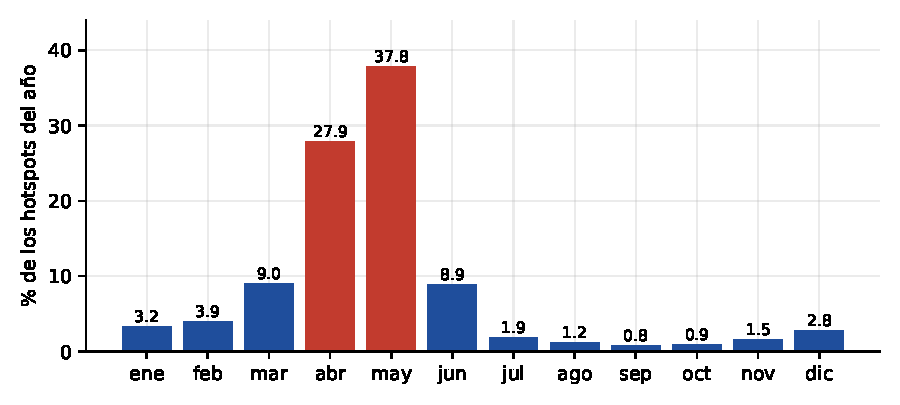
\includegraphics[width=0.85\textwidth]{fig/fig_estacionalidad.pdf}
\caption{Porcentaje de los hotspots equivalentes de cada mes, años 2001--2025 (todos los años juntos). En rojo, abril y mayo.}\label{fig:estacionalidad}
\end{figure}

\begin{ideaclave}[Idea clave del capítulo]
La serie armonizada reproduce a MODIS con error anual nacional de $1.3\,\%$ y $2.1\,\%$, y por estado y mes de $12.9\,\%$ y $14.5\,\%$. Calibrar por estado y mes reduce el error por estado y mes entre un tercio y la mitad frente a un factor único. Fusionar píxeles y filtrar por FRP, que parecían buenas ideas, empeoran el resultado.
\end{ideaclave}

\chapter{El pronóstico}\label{cap:pron}

La aplicación incluye un pronóstico de hotspots equivalentes a MODIS, diario a 30 días, semanal a 12 semanas y mensual a 12 meses, para cualquier estado o para todo México. El modelo es sencillo a propósito: lo que se pueda explicar y verificar en una página pesa más que una promesa de precisión que los datos no sostienen.

\section{Qué se pronostica}

Sea $S_t$ la serie diaria armonizada de una región (\emph{Todo México} o un estado), con $t=0$ el 1 de noviembre de 2000. Elegimos un \textbf{origen} $T_0$, el último día observado. El pronóstico usa solo datos con $t\le T_0$ y entrega, para cada periodo futuro $P$, un valor puntual $\widehat Y_P$ y un intervalo de $80\,\%$.

\begin{itemize}
  \item \textbf{Diario}: los 30 días siguientes, $P=\{T_0+h\}$, $h=1,\dots,30$.
  \item \textbf{Semanal}: 12 bloques de 7 días consecutivos, $P_w=\{T_0+7(w-1)+1,\dots,T_0+7w\}$.
  \item \textbf{Mensual}: los 12 meses calendario siguientes. El primer mes incluye la parte ya observada hasta $T_0$.
\end{itemize}

\section{Paso 1: climatología de la misma fecha}

Para un día futuro $t$, la climatología es el promedio, sobre los $K$ años anteriores, del nivel diario alrededor de esa misma fecha del calendario:
\begin{align}
  c_t&=\frac{\sum_{k=1}^{K}\lambda^{\,k-1}\,\overline S_{t,k}}{\sum_{k=1}^{K}\lambda^{\,k-1}},&
  \overline S_{t,k}&=\frac{1}{2W+1}\sum_{j=-W}^{W}S_{t_k+j},\label{eq:clim}
\end{align}
donde $t_k$ es el mismo día del calendario $k$ años antes (el 29 de febrero se trata como 28 de febrero). La suma solo incluye los años $k$ cuya ventana completa $[t_k-W,\,t_k+W]$ ya fue observada, es decir, que termina en $T_0$ o antes. Si ningún año cumple, se usa el promedio diario de los últimos 365 días.

Los valores finales son $K=12$, $\lambda=1$ (todos los años pesan igual) y $W=14$ días.

\paragraph{Interpretación.} $c_t$ estima el nivel esperado de la temporada en esa fecha. Con $K=12$ y $2W+1=29$, cada $c_t$ promedia hasta $12\times29=348$ valores diarios. Promediar reduce el ruido, que es grande porque cada día es un conteo pequeño. La ventana $W$ tiene un costo: en el pico de la temporada la serie sube y baja con rapidez, y una ventana ancha suaviza el máximo. Es el compromiso clásico entre sesgo y varianza: ventana chica, más ruido; ventana grande, más sesgo en las cimas.

\section{Paso 2: ajuste de nivel reciente}

La climatología supone un año promedio. Pero hay años de mucho y de poco fuego, y el comportamiento reciente dice algo sobre el resto del año. Medimos qué tanto se desvía lo observado en los últimos $L$ días del promedio esperado:
\begin{align}
  r=\min\!\left\{4,\;\max\!\left\{\tfrac14,\;\frac{\sum_{t=T_0-L+1}^{T_0}S_t+c_0}{\sum_{t=T_0-L+1}^{T_0}c_t+c_0}\right\}\right\},\label{eq:r}
\end{align}
con $L=28$ días y $c_0=5$. En el denominador, la climatología de los días pasados $c_t$ se calcula con la misma regla de la ecuación~\eqref{eq:clim} y solo con datos hasta $T_0$; si se pudo calcular en menos de $80\,\%$ de esos días, se toma $r=1$ (sin ajuste), y si faltan algunos días la suma se reescala proporcionalmente.

\paragraph{Por qué una razón de totales con pseudoconteo.} Es la misma idea del capítulo~\ref{cap:factor}: la razón de totales es más estable que el promedio de razones diarias, y el pseudoconteo $c_0$ evita que un periodo con casi nada de fuego (por ejemplo, octubre) produzca una razón enorme por dividir entre un número muy pequeño. El recorte a $[1/4,\,4]$ evita ajustes extremos. Si $r>1$ el mes pasado estuvo más activo que lo normal; si $r<1$, menos.

\section{Paso 3: el ajuste se apaga con el horizonte}

Aplicar $r$ de forma permanente sería un error: que las últimas cuatro semanas hayan estado activas informa sobre las próximas semanas, pero poco sobre dentro de cinco meses. Por eso se desvanece de forma exponencial con el horizonte $h=t-T_0$:
\begin{align}
  \boxed{\;\widehat s_{T_0+h}=c_{T_0+h}\cdot\exp\!\bigl(\ln r\cdot e^{-h/\vartheta}\bigr)=c_{T_0+h}\cdot r^{\,e^{-h/\vartheta}}\;},\qquad\vartheta=60\text{ días}.\label{eq:pron}
\end{align}

Los dos extremos tienen sentido. Para $h$ pequeño, $e^{-h/\vartheta}\approx1$ y $\widehat s\approx c\cdot r$: se persiste el nivel reciente. Para $h$ grande, $e^{-h/\vartheta}\to0$ y $\widehat s\to c$: se regresa a la climatología.

\paragraph{Lectura estadística.} En logaritmos, $\ln(\widehat s/c)=\ln r\cdot e^{-h/\vartheta}=\ln r\cdot\varphi^{h}$ con $\varphi=e^{-1/\vartheta}\approx0.9835$ por día: es la \emph{función de respuesta} de un proceso autorregresivo AR(1) en las desviaciones logarítmicas respecto a la climatología. La vida media del ajuste, el horizonte en que su efecto se reduce a la mitad, es $\vartheta\ln2\approx41.6$ días.

\begin{table}[H]
\centering
\caption{Peso del ajuste de nivel, $e^{-h/\vartheta}$ con $\vartheta=60$.}\label{tab:peso}
\small
\begin{tabular}{@{}lrrrrrr@{}}
\toprule
Horizonte $h$ (días) & 1 & 7 & 30 & 60 & 120 & 180 \\
\midrule
Peso del ajuste & 0.98 & 0.89 & 0.61 & 0.37 & 0.14 & 0.05 \\
\bottomrule
\end{tabular}
\end{table}

\begin{figure}[H]
\centering
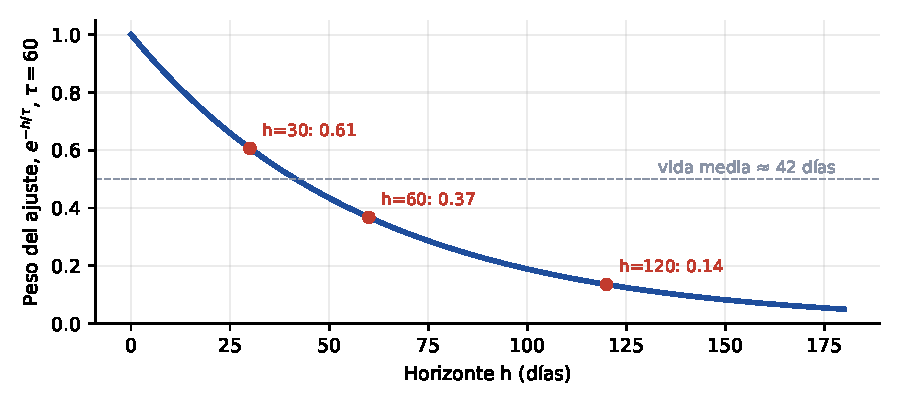
\includegraphics[width=0.82\textwidth]{fig/fig_decaimiento.pdf}
\caption{Peso del ajuste de nivel según el horizonte.}\label{fig:decae}
\end{figure}

\begin{ejemplo}[Cómo se ve con el 2026 de la aplicación]
Con origen el 31 de diciembre de 2025, Todo México sumó $1\,554$ hotspots equivalentes en los últimos 28 días, contra $1\,472$ que daba la climatología: $r\approx1.056$ (con $c_0=5$ casi no cambia). A 30 días el exponente pesa $0.61$ y el ajuste es de $1.056^{0.61}\approx1.033$, o sea $3.3\,\%$ por encima de la climatología. Para mayo (más de 120 días adelante) el exponente pesa menos de $0.14$ y el pronóstico es prácticamente la climatología.
\end{ejemplo}

\section{De la trayectoria diaria a semanas y meses}

El pronóstico de un periodo $P$ es la suma de la parte ya observada y la parte pronosticada:
\begin{align*}
  \widehat Y_P=\underbrace{\sum_{t\in P,\;t\le T_0}S_t}_{\text{observada}}+\underbrace{\sum_{t\in P,\;t>T_0}\widehat s_t}_{\text{pronosticada}}.
\end{align*}
A lo sumo el primer mes calendario tiene parte observada. Al evaluar, el error se mide únicamente en la parte pronosticada, $\widehat Y^{\mathrm{rem}}_P=\sum_{t\in P,\,t>T_0}\widehat s_t$ contra su valor real $Y^{\mathrm{rem}}_P$, para que la parte conocida no regale precisión.

\section{Intervalos de \texorpdfstring{$80\,\%$}{80 \%} con errores del propio modelo}\label{sec:interv}

El intervalo no sale de una distribución supuesta sino de los errores que el modelo \emph{habría cometido} en el pasado.

\paragraph{Error relativo en logaritmos.} Para un origen histórico $T$ y un periodo $P$ con $n_P$ días por pronosticar, definimos
\begin{align*}
  \rho_{T,P}=\ln\frac{Y^{\mathrm{rem}}_{T,P}+\kappa\,n_P}{\widehat Y^{\mathrm{rem}}_{T,P}+\kappa\,n_P},\qquad\kappa=0.5.
\end{align*}
Usamos el cociente y su logaritmo porque el error de un conteo crece con su nivel: equivocarse en 100 hotspots es grave en septiembre y normal en mayo. El pseudoconteo $\kappa\,n_P$ (medio hotspot por día) evita $\ln0$ y el comportamiento errático de los periodos casi vacíos; es la misma estrategia del $c_0$ de la ecuación~\eqref{eq:r}.

\paragraph{Conjunto de errores disponibles.} Se calcula $\rho_{T,P}$ para orígenes semanales desde el 1 de enero de 2003 y para los tres tipos de periodo (día, semana, mes). Para un origen nuevo $T_0$ solo se admiten errores de periodos que \emph{ya terminaron} en $T_0$ o antes (así se evita usar el futuro) y con una estación parecida: la distancia circular en el día del año entre $T$ y $T_0$ debe ser $\le\omega$, con $\omega\in\{45,90,183\}$ días; se toma el menor $\omega$ que deja al menos 40 errores.

\paragraph{Cuantiles y regreso a la escala original.} Sean $q_{10}$ y $q_{90}$ los cuantiles empíricos de $\rho$. El intervalo para la parte pronosticada es
\begin{align*}
  \Bigl[\;\bigl(\widehat Y^{\mathrm{rem}}_P+\kappa n_P\bigr)e^{q_{10}}-\kappa n_P,\;\;\bigl(\widehat Y^{\mathrm{rem}}_P+\kappa n_P\bigr)e^{q_{90}}-\kappa n_P\;\Bigr]_{+},
\end{align*}
donde $[\,\cdot\,]_+$ trunca en 0 el límite inferior; a ambos se les suma la parte observada. El intervalo es multiplicativo y su ancho se adapta a la estación.

\begin{cuidado}[Los intervalos de varios periodos no se suman]
Cada intervalo es de $80\,\%$ para su propio periodo. Sumar los límites de los 12 meses no da un intervalo de $80\,\%$ del total anual: esos errores no son independientes ni tienen el mismo signo. Por eso la aplicación y este documento reportan intervalos por mes, pero no uno del total anual.
\end{cuidado}

\section{Líneas base para comparar}

Un pronóstico solo vale algo frente a otro más simple. Comparamos con:

\begin{enumerate}[label=\arabic*)]
  \item \textbf{Solo climatología}: la ecuación~\eqref{eq:pron} con $r=1$. Aísla la contribución del ajuste de nivel.
  \item \textbf{Mismo periodo del año anterior}: el nivel de la ventana de $\pm14$ días de la misma fecha un año antes ($K=1$, sin ajuste). Es la regla «este año será igual que el pasado».
\end{enumerate}

\section{Elección de los parámetros}

Se exploró una rejilla de $3\times2\times2\times4=48$ combinaciones con $K\in\{4,8,12\}$, $\lambda\in\{1,0.8\}$, $W\in\{7,14\}$ y $\vartheta\in\{0,20,60,150\}$, dejando $L=28$ y $c_0=5$ fijos. El criterio fue el WAPE promedio de los tres niveles (día, semana y mes), promediado con igual peso entre las 33 regiones, con orígenes cada 14 días entre el 1 de enero de 2010 y el 31 de diciembre de 2019. Ganó $K=12$, $\lambda=1$, $W=14$, $\vartheta=60$.

\begin{table}[H]
\centering
\caption{Las cinco mejores combinaciones de la rejilla (WAPE medio entre 33 regiones, \%).}\label{tab:rejilla}
\small
\begin{tabular}{@{}rrrrrrrr@{}}
\toprule
$K$ & $\lambda$ & $W$ & $\vartheta$ & Diario & Semanal & Mensual & Criterio \\
\midrule
\textbf{12} & \textbf{1} & \textbf{14} & \textbf{60} & \textbf{85.0} & \textbf{61.8} & \textbf{51.5} & \textbf{66.1} \\
12 & 0.8 & 14 & 60 & 85.0 & 61.9 & 51.9 & 66.3 \\
12 & 1 & 7 & 60 & 85.5 & 62.5 & 51.6 & 66.5 \\
8 & 0.8 & 14 & 60 & 85.2 & 62.3 & 52.3 & 66.6 \\
12 & 0.8 & 7 & 60 & 85.5 & 62.4 & 51.9 & 66.6

\\
\bottomrule
\end{tabular}
\end{table}

\begin{cuidado}[Dos precisiones]
1) El criterio da el mismo peso a cada región, así que lo domina el desempeño en estados chicos, de errores grandes. 2) $K=12$ y $\lambda=1$ están en el borde de la rejilla: es posible que más años de historia mejoren un poco el pronóstico; no lo exploramos. Además, los periodos objetivo de los últimos orígenes (hasta 12 meses adelante) llegan a 2020, por lo que una fracción pequeña del criterio de ajuste toca ese año.
\end{cuidado}

\section{La prueba hacia atrás}

El modelo se evalúa con \textbf{orígenes semanales del 1 de enero de 2020 al 31 de diciembre de 2025} (314 orígenes). En cada uno se hace el pronóstico con datos hasta ese día, se construyen los intervalos solo con errores ya observables y se compara con lo que ocurrió, para cada región y cada nivel (día, semana, mes). Las métricas son:

\begin{itemize}
  \item \textbf{WAPE} de la parte pronosticada, sumando sobre todos los orígenes y periodos de la región.
  \item \textbf{Sesgo}, $\sum(\widehat Y^{\mathrm{rem}}-Y^{\mathrm{rem}})/\sum Y^{\mathrm{rem}}$.
  \item \textbf{Cobertura} del intervalo de $80\,\%$: proporción de periodos en que lo observado cae dentro del intervalo.
\end{itemize}

\begin{cuidado}[Muestras que se traslapan]
Los pronósticos de orígenes consecutivos se traslapan (la semana siguiente repite casi todo el horizonte), de modo que los errores están correlacionados y el tamaño de muestra efectivo es mucho menor que el número de pares origen--periodo. Por eso no reportamos errores estándar y evitamos dar importancia a diferencias de pocas décimas.
\end{cuidado}

\section{Resultados}

\subsection{Todo México}

\begin{table}[H]
\centering
\caption{Prueba hacia atrás 2020--2025, Todo México. WAPE (\%) del modelo, de la climatología y del año anterior; sesgo del modelo (\%) y cobertura del intervalo de $80\,\%$ (\%).}\label{tab:pron-nac}
\small
\begin{tabular}{@{}lrrrrr@{}}
\toprule
Horizonte & Modelo & Clim. & Año ant. & Sesgo & Cobertura \\
\midrule
Diario (1--30 días) & 30.9 & 31.3 & 37.3 & 2.9 & 85.3 \\
Semanal (1--12 semanas) & 24.8 & 24.3 & 31.3 & 3.6 & 88.8 \\
Mensual (1--12 meses) & 17.9 & 17.5 & 26.1 & 4.9 & 88.7

\\
\bottomrule
\end{tabular}
\end{table}

Lo que dicen los números:

\begin{enumerate}[label=\arabic*)]
  \item El modelo \textbf{supera con claridad} a «igual que el año pasado»: $30.9$ contra $37.3\,\%$ diario, $24.8$ contra $31.3\,\%$ semanal y $17.9$ contra $26.1\,\%$ mensual.
  \item El modelo \textbf{empata con la climatología}: es algo mejor a un día ($30.9$ contra $31.3\,\%$) y algo peor a semanas y meses ($24.8$ contra $24.3\,\%$ y $17.9$ contra $17.5\,\%$). Dadas las muestras que se traslapan, no distinguimos estas diferencias.
  \item El modelo \textbf{sobrestima ligeramente}: entre $+2.9$ y $+4.9\,\%$. No investigamos la causa.
  \item Los intervalos \textbf{cubren más que lo nominal}: entre $85$ y $89\,\%$ para un nivel de $80\,\%$. Son algo anchos.
\end{enumerate}

\begin{figure}[H]
\centering
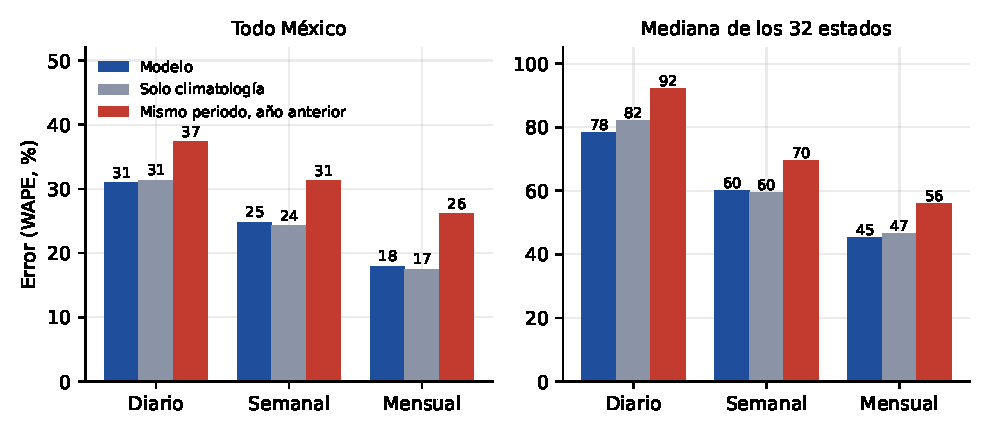
\includegraphics[width=0.98\textwidth]{fig/fig_error_pron.pdf}
\caption{Error de la prueba hacia atrás 2020--2025. Izquierda, Todo México; derecha, mediana de los 32 estados.}\label{fig:error-pron}
\end{figure}

\subsection{Por estado}

\begin{table}[H]
\centering
\caption{Prueba hacia atrás 2020--2025, mediana de los 32 estados. Error mediano (\%) y número de estados (de 32) en que el modelo supera al año anterior y a la climatología.}\label{tab:pron-est}
\small
\begin{tabular}{@{}lrrrrrr@{}}
\toprule
Horizonte & Modelo & Clim. & Año ant. & $<$ año ant. & $<$ clim. & Cobertura \\
\midrule
Diario (1--30 días) & 78.4 & 82.0 & 92.2 & 29 & 22 & 85.2 \\
Semanal (1--12 semanas) & 60.1 & 59.6 & 69.7 & 29 & 26 & 81.7 \\
Mensual (1--12 meses) & 45.3 & 46.6 & 56.1 & 26 & 26 & 82.2

\\
\bottomrule
\end{tabular}
\end{table}

Por estado el error es mucho mayor (mediana de $78\,\%$ diario, $60\,\%$ semanal y $45\,\%$ mensual), sobre todo en estados con pocos hotspots, donde cada día es casi un conteo de cero o uno. El modelo supera al año anterior en 29, 29 y 26 de los 32 estados, y a la climatología en 22, 26 y 26. La cobertura mediana de los intervalos por estado está entre $82$ y $85\,\%$, cercana a lo nominal.

\section{El pronóstico de 2026}

Con origen el 31 de diciembre de 2025, el modelo anticipa para 2026 unos 58.6 mil hotspots equivalentes en México, \crec{}\,\% más que los 52.4 mil de la serie de 2025, con el máximo en mayo (figura~\ref{fig:pron2026}; la tabla~\ref{tab:pron2026} está en el anexo).

\begin{figure}[H]
\centering
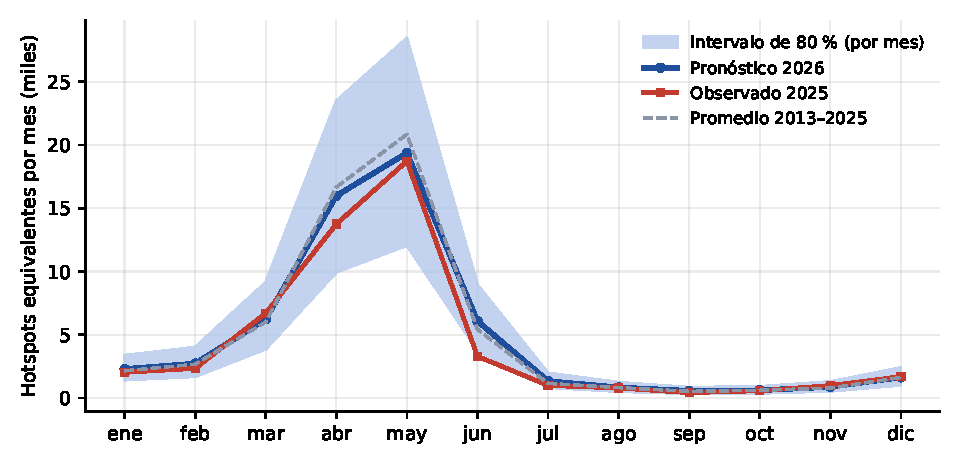
\includegraphics[width=0.95\textwidth]{fig/fig_pron2026.pdf}
\caption{Pronóstico mensual de 2026 para México, con intervalos de $80\,\%$ para cada mes, frente a lo observado en 2025 y al promedio 2013--2025.}\label{fig:pron2026}
\end{figure}

\begin{cuidado}[2026 no se pudo verificar]
Nuestros datos terminan el 31 de diciembre de 2025. No hay forma de comparar este pronóstico con lo que ocurrió en 2026 con la información del proyecto. La prueba hacia atrás dice qué tan bien funcionó el método en 2020--2025; no garantiza nada sobre 2026. En la aplicación se puede escoger un origen anterior y ver el pronóstico contra lo observado.
\end{cuidado}

\begin{ideaclave}[Idea clave del capítulo]
El pronóstico es climatología más un ajuste de nivel que se apaga con el horizonte (ecuación~\eqref{eq:pron}), con intervalos tomados de sus propios errores pasados. A escala nacional empata con la climatología y gana con claridad a repetir el año anterior. Es una línea base estacional con incertidumbre cuantificada, no una predicción de incendios.
\end{ideaclave}

\chapter{Límites y amenazas a la validez}\label{cap:limites}

Un buen análisis dice dónde puede fallar. Esta es la lista que debemos tener presente al presentar el proyecto, ordenada de lo más importante a lo más técnico.

\begin{enumerate}[label=\arabic*.]
  \item \textbf{Un hotspot no es un incendio ni una superficie quemada.} Un incendio grande genera muchos hotspots y un fuego pequeño puede generar uno o ninguno. La serie mide detecciones térmicas de satélite, y no hectáreas ni daños.

  \item \textbf{Validamos contra MODIS, no contra la realidad.} La armonización consiste en reproducir el conteo que habría dado MODIS. Si MODIS tiene sesgos (nubes, hora de paso, fuegos pequeños que no ve), la serie armonizada los hereda.

  \item \textbf{El factor se supone estable en el tiempo.} El modelo de la sección~\ref{sec:modelo} supone que la relación entre sensores no cambia entre años. Los resultados de 2020--2025 son compatibles con esa estabilidad (sesgo de $+0.39\,\%$), pero cualquier cambio en la hora de paso o en el desempeño de los satélites la rompería. Terra y Aqua ya no mantienen su órbita original y su hora de paso cambia con los años (información pública de la NASA que no verificamos con los datos de este proyecto); no lo modelamos.

  \item \textbf{La etapa 2000--2002 es una extrapolación hacia atrás.} Su factor de Terra se calibró con 2003--2011 (sección~\ref{sec:terra}), y no hay con qué compararla.

  \item \textbf{Los conteos reales están sobredispersos.} Las fórmulas de varianza del capítulo~\ref{cap:factor} suponen Poisson e independencia, y los fuegos se agrupan en el espacio y el tiempo. Son una referencia de orden de magnitud: la incertidumbre real es mayor.

  \item \textbf{Elecciones que miraron los datos de prueba.} El parámetro $\tau$ de la contracción se escogió mirando ambos ejercicios, incluido 2020--2025 (sección~\ref{sec:tau}); y los periodos objetivo de los últimos orígenes del ajuste del pronóstico llegan a 2020. El efecto es pequeño en ambos casos, pero la prueba no es perfectamente virgen. Además, $K=12$ y $\lambda=1$ están en el borde de la rejilla del pronóstico.

  \item \textbf{Las pruebas del pronóstico se traslapan.} Los orígenes semanales tienen horizontes que se superponen, así que las muestras no son independientes y no damos errores estándar. Diferencias de décimas de punto entre el modelo y la climatología no son interpretables.

  \item \textbf{El pronóstico no usa clima ni otras variables.} Es un modelo de conteos que repite la estacionalidad con un ajuste de nivel. No incorpora sequía, temperatura, humedad ni El Niño, que sí influyen en la actividad de un año. El pronóstico de 2026 no se pudo verificar.

  \item \textbf{Errores grandes en escalas pequeñas.} Por estado el error mediano del pronóstico es de $45$ a $78\,\%$, y en estados con pocos hotspots puede pasar de $100\,\%$. Las celdas de $0.25^\circ$ de la aplicación tienen más dispersión aún; hay que leer rectángulos pequeños con cautela.

  \item \textbf{Cobertura de datos.} Solo se usaron MODIS (Terra y Aqua) y VIIRS S-NPP hasta el 31 de diciembre de 2025. No entran VIIRS NOAA-20 ni NOAA-21, ni los datos de 2026 en tiempo casi real.
\end{enumerate}

\begin{ideaclave}[Cómo presentar estos límites]
Decirlos de frente fortalece el proyecto. Los números que sí afirmamos (error anual de $1$ a $2\,\%$, error por estado y mes de $13$ a $15\,\%$, pronóstico nacional a la par de la climatología) salen de pruebas con datos que el método no usó, y cada uno trae una condición que ya está dicha en este capítulo.
\end{ideaclave}

\chapter{Cómo reproducir los resultados}\label{cap:repro}

Todo está en el paquete \texttt{calendario\_quemas}. La tabla~\ref{tab:scripts} relaciona cada parte de este documento con el código que la produce.

\begin{table}[H]
\centering
\caption{Dónde está el código de cada parte.}\label{tab:scripts}
\small
\begin{tabularx}{\textwidth}{@{}lXl@{}}
\toprule
Capítulo & Qué hace & Archivo \\
\midrule
\ref{cap:datos} & Carga los parquet de FIRMS y unifica el esquema de MODIS y VIIRS & \texttt{pipeline/01\_load.py} \\
\ref{cap:datos} & Filtra (tipo 0, confianza nominal o alta) y asigna estado & \texttt{pipeline/03\_footprints.py} \\
\ref{cap:factor}, \ref{cap:serie} & Calcula los factores $\widetilde k$ y las series armonizadas & \texttt{pipeline/07\_build.py} \\
\ref{cap:valid}, \ref{cap:result} & Un año fuera, años no vistos, variantes y Terra a Terra más Aqua & \texttt{pipeline/08\_validation.py} \\
\ref{sec:tau} & Búsqueda del parámetro $\tau$ (experimentos) & \texttt{pipeline/05\_experiment2.py} \\
\ref{cap:pron} & Motor del pronóstico (el mismo en el navegador y en Node) & \texttt{app/forecast.js} \\
\ref{cap:pron} & Rejilla de parámetros con orígenes 2010--2019 & \texttt{pipeline/11\_pronostico\_ajuste.js} \\
\ref{cap:pron} & Prueba hacia atrás 2020--2025 & \texttt{pipeline/12\_pronostico\_validacion.js} \\
\ref{cap:pron} & Pronóstico desde el 31 de diciembre de 2025 & \texttt{pipeline/13\_pronostico\_exportar.js} \\
\bottomrule
\end{tabularx}
\end{table}

\section{Comandos}

Para los datos y la validación se requiere Python 3 con \texttt{pandas}, \texttt{numpy}, \texttt{pyarrow}, \texttt{geopandas} y \texttt{shapely}:
\begin{verbatim}
python3 pipeline/01_load.py <carpeta_con_parquet> data/all_points.parquet
python3 pipeline/03_footprints.py data/all_points.parquet \
        geo/mex_adm1_full.geojson data/points_state.parquet
python3 pipeline/07_build.py data/points_state.parquet \
        geo/mex_adm1_full.geojson out
python3 pipeline/08_validation.py data/points_state.parquet \
        out/app_data/validacion.json
\end{verbatim}

Para el pronóstico se requiere Node.js y un archivo \texttt{series.json} con un valor diario por región desde el 1 de noviembre de 2000 (la serie \texttt{hotspots\_armonizados\_estado\_dia.csv}, sumada para «Todo México»):
\begin{verbatim}
node pipeline/11_pronostico_ajuste.js     series.json
node pipeline/12_pronostico_validacion.js series.json \
     datos_armonizados/validacion_pronostico.csv app/data/validacion.json
node pipeline/13_pronostico_exportar.js   series.json \
     datos_armonizados/pronostico_desde_2025-12-31.csv
\end{verbatim}

\section{Verificación independiente de las cifras de este documento}

Las cifras de validación del capítulo~\ref{cap:result} se reprodujeron, además, de forma independiente a partir de los CSV publicados (\texttt{hotspots\_armonizados\_estado\_mes.csv}): se reconstruyen los arreglos $M$, $V$ y $T$, se vuelve a calibrar y se recalcula el WAPE. Coinciden con \texttt{validacion.json} hasta la cuarta cifra decimal, y la tabla~\ref{tab:tau} sale de ese mismo cálculo. Las tablas y las cifras de este documento se generan con un script a partir de los archivos del paquete (\texttt{repro\_validacion.py} y \texttt{gen\_tablas.py}, incluidos con el código fuente de este documento).

\begin{ideaclave}[Idea clave del capítulo]
Cada número de la presentación y de este documento se puede regenerar con los scripts del paquete. El único paso que no se puede repetir sin acceso a internet es la descarga de los parquet de FIRMS y de los contornos de geoBoundaries.
\end{ideaclave}

\appendix
\chapter{Tablas de apoyo}

\section{Factores nacionales por mes}

La tabla~\ref{tab:knat} contiene los factores nacionales que sirven de centro de la contracción (ecuación~\eqref{eq:ktilde}). La columna $1/\widehat k^{V}_{\mathrm{nac}}$ dice cuántas detecciones de VIIRS equivalen a un hotspot de MODIS.

\begin{table}[H]
\centering
\caption{Factores nacionales. $\widehat k^{V}_{\mathrm{nac}}$ se calibró con 2012--2019 (sin enero de 2012) y $\widehat k^{T}_{\mathrm{nac}}$, con 2003--2011.}\label{tab:knat}
\small
\begin{tabular}{@{}lrrr@{}}
\toprule
Mes & $\widehat k^{V}_{\mathrm{nac}}$ & $1/\widehat k^{V}_{\mathrm{nac}}$ & $\widehat k^{T}_{\mathrm{nac}}$ \\
\midrule
Enero & 0.292 & 3.42 & 2.574 \\
Febrero & 0.265 & 3.78 & 2.484 \\
Marzo & 0.263 & 3.81 & 2.590 \\
Abril & 0.284 & 3.52 & 2.232 \\
Mayo & 0.247 & 4.04 & 2.125 \\
Junio & 0.195 & 5.14 & 2.145 \\
Julio & 0.221 & 4.52 & 2.176 \\
Agosto & 0.242 & 4.13 & 2.189 \\
Septiembre & 0.302 & 3.31 & 2.066 \\
Octubre & 0.270 & 3.70 & 2.098 \\
Noviembre & 0.251 & 3.98 & 2.340 \\
Diciembre & 0.306 & 3.27 & 2.606

\\
\bottomrule
\end{tabular}
\end{table}

\section{Pronóstico mensual de 2026 para México}

\begin{table}[H]
\centering
\caption{Pronóstico desde el 31 de diciembre de 2025 (hotspots equivalentes a MODIS). El intervalo de $80\,\%$ es de cada mes por separado; el total no lleva intervalo (véase la sección~\ref{sec:interv}). Se incluyen el observado de 2025 y el promedio 2013--2025 como referencia.}\label{tab:pron2026}
\small
\begin{tabular}{@{}lrrrr@{}}
\toprule
Mes & Pronóstico & Intervalo de 80\,\% & Observado 2025 & Promedio 2013--2025 \\
\midrule
Enero 2026 & 2\,298 & 1\,426--3\,382 & 2\,031 & 2\,154 \\
Febrero 2026 & 2\,732 & 1\,697--4\,020 & 2\,346 & 2\,679 \\
Marzo 2026 & 6\,226 & 3\,873--9\,150 & 6\,709 & 6\,011 \\
Abril 2026 & 15\,987 & 9\,956--23\,486 & 13\,755 & 16\,669 \\
Mayo 2026 & 19\,372 & 12\,065--28\,457 & 18\,724 & 20\,844 \\
Junio 2026 & 6\,088 & 3\,788--8\,948 & 3\,302 & 5\,429 \\
Julio 2026 & 1\,346 & 833--1\,984 & 999 & 1\,161 \\
Agosto 2026 & 844 & 520--1\,246 & 797 & 826 \\
Septiembre 2026 & 574 & 352--850 & 427 & 532 \\
Octubre 2026 & 617 & 379--914 & 580 & 618 \\
Noviembre 2026 & 882 & 544--1\,303 & 991 & 793 \\
Diciembre 2026 & 1\,639 & 1\,015--2\,414 & 1\,696 & 1\,632 \\
\midrule
Total & 58\,605 & --- & 52\,357 & 59\,348

\\
\bottomrule
\end{tabular}
\end{table}

\chapter{Preguntas que puede hacer el jurado}

Cada respuesta es corta y señala dónde está el sustento en este documento.

\begin{description}[leftmargin=1em,style=nextline,itemsep=8pt]
  \item[¿Por qué no basta un solo factor para todo México?]
  Porque la razón entre sensores cambia con el mes y con el estado (figura~\ref{fig:knat}). Con un factor único el error por estado y mes es de $24.8\,\%$ y $21.3\,\%$; con factor por estado y mes baja a $12.9\,\%$ y $14.5\,\%$ (tabla~\ref{tab:niveles}).

  \item[¿Cómo sabemos que no está ajustado a los datos que usamos para medir?]
  Medimos con dos ejercicios en los que el año evaluado no entra al cálculo del factor: dejar un año fuera (2012--2019) y predecir 2020--2025, años que el método no usó (capítulo~\ref{cap:valid}). El único parámetro que miró ambos es $\tau$, y su efecto es de décimas de punto (sección~\ref{sec:tau}).

  \item[¿Por qué una razón de totales y no un promedio de razones?]
  Porque es el estimador de máxima verosimilitud condicional bajo un modelo de Poisson y no necesita modelar la intensidad del fuego de cada año (sección~\ref{sec:est-razon}); además da más peso a los años con más datos.

  \item[¿Qué es la contracción y por qué $\tau=100$?]
  Es una media ponderada entre el factor del estado y el nacional del mismo mes, con peso $\sum V/(\sum V+\tau)$ para el estado; equivale a una media a posteriori beta--binomial (sección~\ref{sec:contraccion}). El error es casi igual entre $\tau=30$ y $\tau=300$ (tabla~\ref{tab:tau}).

  \item[¿Por qué descartaron fusionar píxeles de VIIRS y filtrar por FRP?]
  Porque empeoraron todas las métricas (tabla~\ref{tab:variantes}); el error anual fuera de muestra pasó de $2.1\,\%$ a entre $4.4\,\%$ y $7.6\,\%$.

  \item[¿Qué tan confiable es la parte de 2000--2002?]
  Es la más incierta: el factor de Terra se calibró con 2003--2011 y se aplica hacia atrás sin posibilidad de comprobarlo (sección~\ref{sec:terra}).

  \item[¿El pronóstico mejora a la climatología?]
  A escala nacional no de manera apreciable (tabla~\ref{tab:pron-nac}); sí supera con claridad a repetir el año anterior. Por estado supera a la climatología en 22 a 26 de los 32 estados según el horizonte, con diferencias medianas pequeñas (tabla~\ref{tab:pron-est}).

  \item[¿El pronóstico de 2026 es correcto?]
  No se puede saber con nuestros datos, que terminan en diciembre de 2025. Lo que sí se midió es el desempeño del método de 2020 a 2025 (capítulo~\ref{cap:pron}).

  \item[¿Por qué los intervalos cubren más de $80\,\%$?]
  A escala nacional cubren de $85$ a $89\,\%$: son algo conservadores. Por estado la cobertura mediana es de $82$ a $85\,\%$, más cercana a lo nominal.

  \item[¿Un hotspot es una hectárea quemada?]
  No. Es un píxel con anomalía térmica; no mide superficie quemada ni daño (capítulo~\ref{cap:limites}).
\end{description}

\chapter{Glosario}

\begin{description}[leftmargin=1em,style=nextline,itemsep=6pt]
  \item[Armonizar.] Llevar los conteos de dos sensores a una unidad común de modo que sean comparables.
  \item[Climatología.] Promedio histórico de una variable para la misma fecha del calendario.
  \item[Contracción.] Acercar una estimación ruidosa hacia un valor de referencia más estable, con un peso que depende de la cantidad de datos.
  \item[FIRMS.] Sistema de la NASA que distribuye detecciones de fuego activo casi en tiempo real.
  \item[FRP.] Potencia radiativa del fuego, en megavatios.
  \item[Hotspot.] Píxel de satélite con anomalía térmica compatible con fuego activo.
  \item[Hotspot equivalente a MODIS.] Unidad común de la serie armonizada: lo que habrían contado Terra y Aqua.
  \item[LOYO.] Validación cruzada que deja un año fuera (\emph{leave-one-year-out}).
  \item[Origen.] Último día observado a partir del cual se pronostica.
  \item[Sesgo.] Tendencia sistemática de un método a sobrestimar o subestimar.
  \item[Sobredispersión.] Variabilidad de los conteos mayor que la de un modelo de Poisson.
  \item[WAPE.] Error porcentual absoluto ponderado: suma de errores absolutos entre suma de lo observado.
\end{description}


\end{document}
